\documentclass{homework}

\usepackage{tcolorbox}
\usepackage{etoolbox}
\usepackage{svg}
\usepackage{algorithm}
\usepackage{algpseudocode}
\usepackage{caption}
\usepackage[newfloat]{minted}
\usepackage{pgfplots}
\usepackage{tabularx}
\pgfplotsset{width=10cm,compat=1.9}
\usepackage[super]{nth}
\usepackage{awesomebox}
\usepackage{environ}
\usepackage{tikz}
\usetikzlibrary{fit,backgrounds,calc}
\usepackage{dirtree}
\usepackage[linguistics]{forest}
\usepackage[showframe]{geometry}

\makeatletter                                       
\newenvironment{chapquote}[3][2.7em]
  {\setlength{\@tempdima}{#1}
   \ifx\relax#2\relax\setlength{\@tempdimb}{#1}\else\setlength{\@tempdimb}{#2}\fi
   \def\chapquote@author{#3}
   \parshape 1 \@tempdima \dimexpr\textwidth-\@tempdima-\@tempdimb\relax
   \itshape}
  {\newline\par\normalfont\hfill--\ \chapquote@author\hspace*{\@tempdimb}\par\bigskip}
\makeatother
\begin{document}
\title{Final Project}
\author{32172917 Dabin Lee / 32190984 Isu Kim}
\maketitle

\newminted{python}{frame=lines,framerule=2pt}
\newenvironment{code}{\captionsetup{type=listing}}{}
\SetupFloatingEnvironment{listing}{name=Code Snippet}

\maketitle
\begin{center}
Left Free Days : 5
\end{center}
\pagebreak

\section{Index}
\begin{enumerate}
   \item Virtual memory (Project 2)
   \item File System Background
   \item Compiling and Building
   \item Design \& Sketch
   \item Implementation and Usage
   \item Future Idea \& Conclusion
\end{enumerate}
\pagebreak

\setcounter{section}{0}
\section{Virtual Memory Concepts (Project 2)}
\subsection{Virtual Memory}
As we saw in the previous project, in order to run a program, the program on disk must be in a "process" state loaded into memory. That is, \textit{the instructions currently executing must exist in physical memory}. The easiest way to satisfy this requirement is to put the entire process in memory. However, this method is not good because it limits the size of the program to the size of physical memory. In fact, in many cases, the entire program doesn't need to be in memory all at once.

\textit{So, what are the benefits of running only a portion of a program in memory?} First, programs are no longer constrained by the size of physical memory. Second, each program takes up less memory, allowing more programs to run at the same time. As a result, the response time does not increase, but CPU utilization and throughput increase. Finally, programs run faster because the number of I/Os required to put and swap programs into memory is reduced.

\begin{figure}[h]
\begin{center}
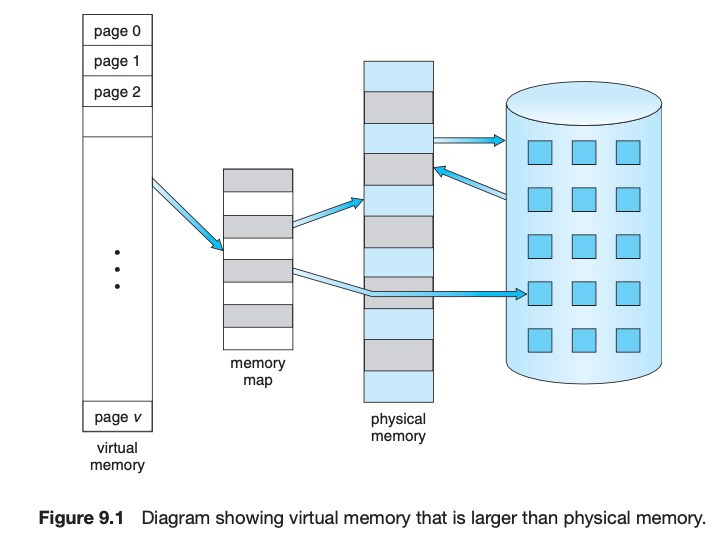
\includegraphics[scale=0.7]{31.png}    
\caption{Virtual Memory Diagram}
\end{center}
\end{figure}

Virtual memory is a separation between the actual physical memory concept and the developer's concept of virtual memory. The advantage of it is that a small amount of memory can provide the programmer with as much virtual address space. Virtual memory makes it easy for programmers to write programs without having to worry about memory size issues. In addition, virtual memory allows files and memory to be shared by two or more processes through page sharing. 

\subsection{Virtual address}

\begin{figure}[h]
\begin{center}
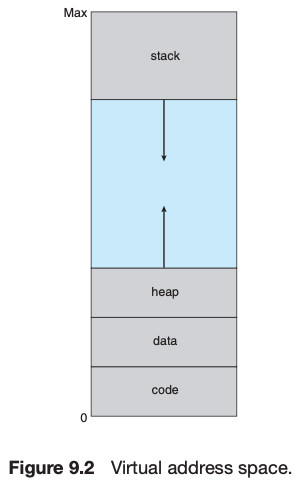
\includegraphics[scale=0.7]{32.png}    
\caption{Virtual Address Space}
\end{center}
\end{figure}

The virtual address space of a process is the logical (or virtual) appearance of how a process is stored in memory. In general, it starts at a specific virtual address (usually address zero) and occupies a \textit{contiguous space}, as shown in the figure above. 
The virtual address space of each process is divided. A 32-bit process can have 4 GB of virtual address space. However, users don't have access to all 4GB of virtual address space, only about 2GB. The reason is that the 32-bit address space is divided as follows:

\begin{itemize}
    \item Null-pointer allocation partition: \textttt{0x00000000~0x0000FFFF}
    \item User Mode Partition: \texttt{0x00010000 ~ 0x7FFEFFFF}
    \item 64KB no-access partition: \texttt{0x7FFF0000~0x7FFFFFF}
    \item Kernel mode partition: \texttt{0x80000000~0xFFFFFFFF}
\end{itemize}

\subsection{Paging}
Paging is a \textit{non-contiguous allocation} method. As a method of solving the inefficiencies of the compaction of external fragmentation, breaking physical memory into fixed-sized blocks called \textit{frames} and breaking logical memory into blocks of the same size called \textit{pages}. In this way, we'll be able to store a page in one frame. 

The space used by a process is divided into several pages, and each page is mapped and stored in a frame in memory in any order. Since processes are not stored in memory in order, we need to know which frame the page is in in order to execute the process. This information is stored in a table called \textit{page table}, which is used to convert logical addresses to physical addresses. Now that the concept of page tables is complete, it is time to map the physical page frame to the virtual page depends on the MMU. In other words, to access memory, it must be accessed by converting a logical address to a physical address through a memory management unit (MMU).

This paging technique has the advantages of being able to solve the problem of external fragmentation, fast allocation and deallocation, and simple swap out, but the disadvantages still do not solve internal fragmentation, additional memory for storing the page table is consumed, and since the page table resides in memory, the access operation is performed twice, which slows down memory access. Therefore, it uses a high-speed hardware cache called \textit{TLB} (Translation Look-aside Buffer) to improve speed.

\begin{figure}[h]
\begin{center}
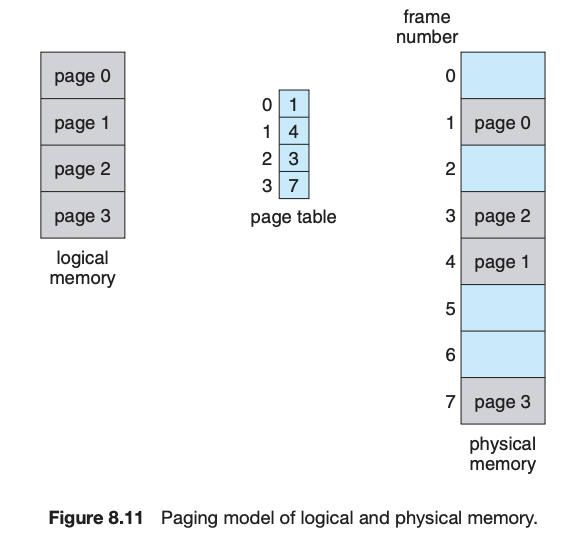
\includegraphics[scale=0.7]{33.png}    
\caption{Paging Model}
\end{center}
\end{figure}
\pagebreak
\subsection{Demand Paging}
Given the nature of paging described above, it seems that there is no need to load all pages into memory. If only the pages that are essential to run the process are loaded into memory at the right time, there will be no big problem in executing the process. This technique is called demand paging. This increases CPU utilization and throughput, and allows for more users.
Demand paging uses a valid-invalid bit in the page table that indicates whether the page is in memory. If bit is invalid, the page is not in physical memory. Therefore, if all page entries are initialized to invalid, and if bit is invalid during address translation, a page fault error occurs. 
The specific process of address conversion is as follows:

\begin{enumerate}
    \item The hardware checks the TLB.
    \item If it is a TLB hit, immediately convert the address, and if it is a TLB miss, check the page table (→3). 
    \item If the valid-invalid bit of the page table is valid, convert the address and add page to the TLB. If invalid, a page fault occurs (→4).
    \item When a page fault occurs, the MMU traps the operating system and enters kernel mode, causing the page fault handler to be invoked.
    \item If the reference is invalid, terminate the process, otherwise get an empty page frame. If there is no empty frame, select a victim page from memory to replace it.  
    \item The operating system loads the referenced page from disk into memory, and this process deprives the CPU until disk I/O ends.
    \item When disk I/O is finished, the page table is updated and the valid-invalid bit is changed to valid. Then put the process in the ready queue. 
    \item When the process catches the CPU, it continues again.
\end{enumerate}

\begin{figure}[h]
\begin{center}
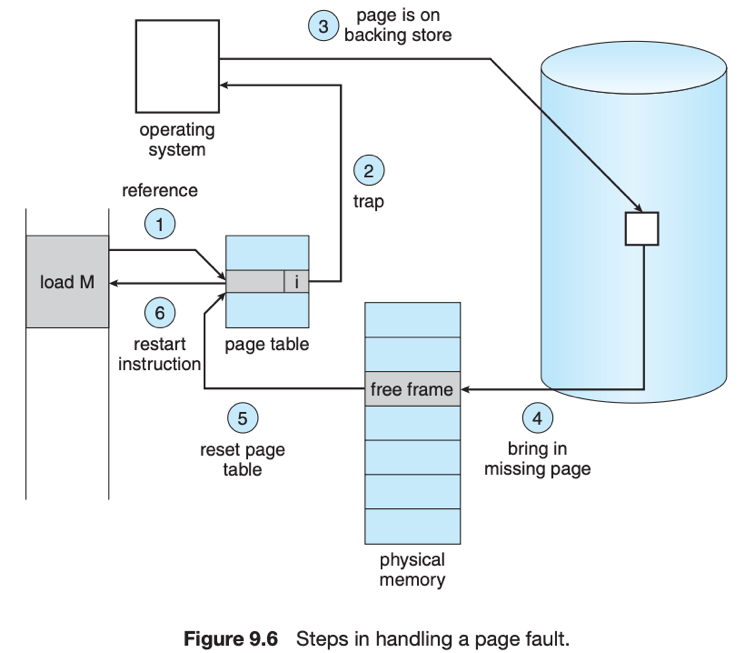
\includegraphics[scale=0.7]{34.png}    
\caption{Demand Paging}
\end{center}
\end{figure}
\pagebreak

\subsection{Page Replacement Algorithm}
As in step 5 of address conversion described above, what if the physical memory is full? One of the existing pages must be stored from physical memory to disk and a new page must be placed in that physical memory. At this time, the page replacement policy is about which page to be demoted from physical memory to the disk, that is, to find the victim page.
\begin{itemize}
    \item \textbf{FIFO (First-In-First-Out)}: FIFO algorithms are a way to kick out what comes in first. You can use it even if you don't know the future. The advantage is that all pages live in the frame equally, and it is easy to implement. However, some pages may always be needed, and even in that case, there is a disadvantage that it is replaced.
    \item \textbf{LRU (Least-Recent-Used)}: The LRU algorithm is a way to erase the oldest references. It is the most optimized page replacement algorithm, but it is difficult to implement, and each time a process accesses main memory, it must record the time for the referenced page. Therefore, large overhead can be incurred.
\end{itemize}

\pagebreak
\section{File System Background}
\subsection{Project Introduction}
This project implements a file system, which reads and mounts the \textit{disk.img} file after all implementations are completed. After that, 10 file names are randomly assigned, and the output is the data of the file name according to the correct structure. In detail, the goal of this project is to print out all the information of the mounted super block and the inode table, and check whether the desired file is loaded correctly. In addition, the goal of this project is to add a write function so that the data in the file can be modified with the data desired by the user.

To implement the project, we must understand the concept, structure, features, and role of the file and the file system and think about why a file system is necessary. Also, by studying the representative types of file systems we understand the overall theory of file systems. Based on this, we can implement open, read, and write that works on the actual file system, and implements the file system based on thinking about how to create additional directories and use shared files by multiple users. Based on this, we will implement open, read, and write that run on the actual file system, and think about how to create additional directories and use files shared by multiple users. Through these efforts, let's implement a complete file system.

\subsection{Concepts}
\subsubsection{File and File System}
\textit{File} is a logical storage unit that gives a name to a set of related information materials (data or programs). It provides a uniform logical perspective of information storage for convenient use of computer systems. It is generally stored in nonvolatile disk memory in record or block units.

\textit{A file system} is a system that stores or organizes files stored on such disks so that they can be easily found and accessed.
To use a simple analogy, a hard disk can be thought of as a library, a file system as a book search table, files as books, and data as the contents of books. So, in order to find the file containing the data you want, there is a file system inside the hard disk.
\subsubsection{File Attributes and Operations}
The attributes of the file vary by operating system, but are usually organized as follows:
\begin{itemize}
    \item \textbf{Name}: Only information in human-readable form.
    \item \textbf{Identifier}: Unique tag that identifies the file within the file system.
    \item \textbf{Location}: Pointer to file location.
    \item \textbf{ETC}: Type, Size, Time, date, and user identification.
\end{itemize}

This information about all files is kept in the directory structure that also resides on secondary storage. A directory entry usually consists of the file’s name and its unique identifier. This identifier is in turn used to find other file attributes.

A file is an abstract data type. So, to define a file we need to know its operations. File performs \textit{create, write, read, reposition within a file, delete, truncate}. These six basic operations consist of the minimal set of required file operations.

\subsubsection{Directory and Disk Structure}
Typically, thousands to billions of files are stored on random access devices such as hard disks. Since there are too many files to be saved, it is necessary to build a system for saving files. This entails the use of \textit{directories}. The directory determines the overall structure of the file system by associating the name of each file with the file itself.
\begin{itemize}
    \item \textbf{Volume}: storage area on disk formatted with a filesystem, disks are segmented into one or more volumes, each containing a file system or left raw(unformatted disk space).
    \item \textbf{Device directory}: records information such as name, location, size, and type for all files on that volume.
    \item \textbf{Partition}: a protocol defined so that contiguous storage space can be divided into one or more contiguous and independent areas. It's common to have multiple partitions on a single physical disk.
\end{itemize}

\begin{figure}[h]
\begin{center}
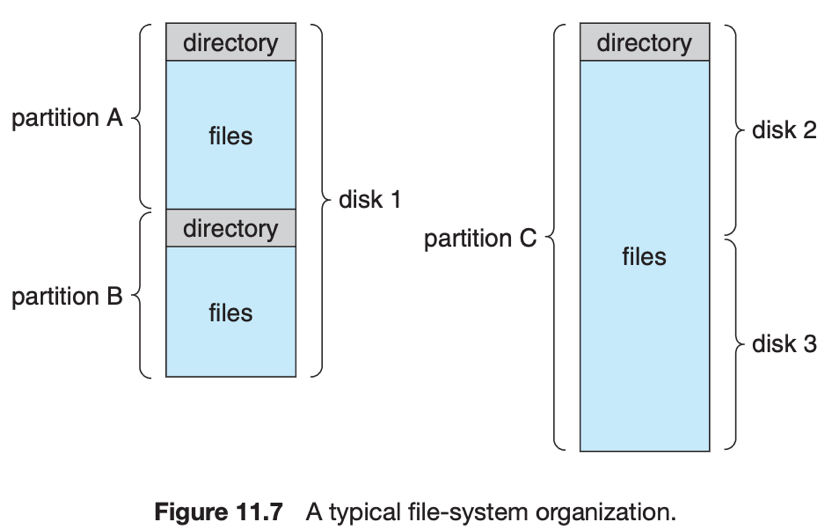
\includegraphics[scale=0.7]{35.png}    
\caption{File System Organization}
\end{center}
\end{figure}

\begin{itemize}
    \item \textbf{Tree-Structured Directories}: the tree structure allows users to create their own subdirectories and organize files accordingly. It has one root directory and several sub-directories. Also, every file on the system has its own path. This allows for efficient navigation and grouping. Since a directory is a type of file, it is necessary to distinguish whether it is a file or a directory. Each entry in the directory uses one bit to distinguish whether it is a file (0) or a directory file (1). And all directories have the same internal format.
\end{itemize}

\begin{figure}[h]
\begin{center}
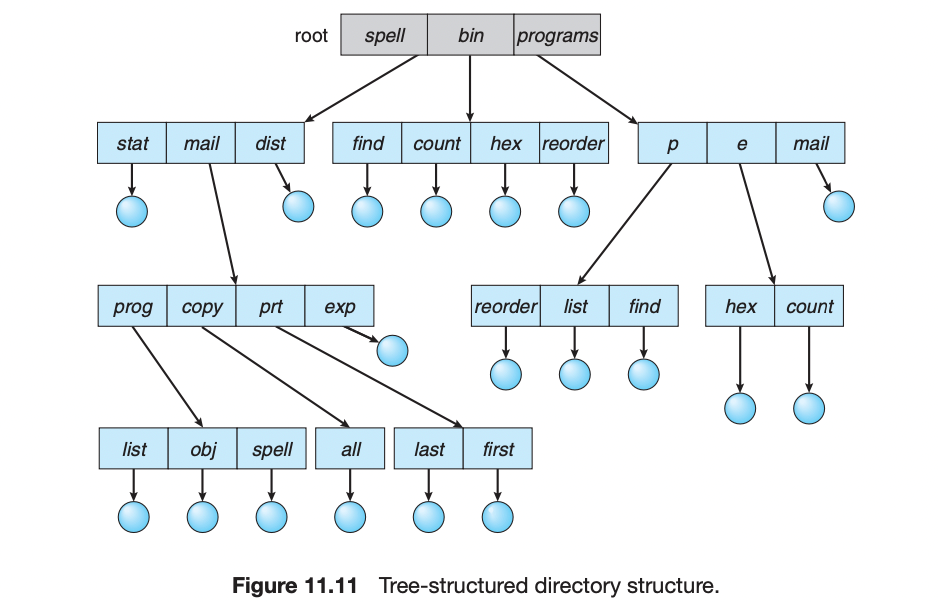
\includegraphics[scale=0.7]{36.png}    
\caption{Tree Structured Directory}
\end{center}
\end{figure}

\subsubsection{File-System Mounting}
The operation performed before the file is used, the file system must be mounted before it can be used by processes. That is, the operating system is given the name and file location of the device. Typically, a mount point is an empty directory where the file system will be attached. The operating system verifies that the device contains a valid file system. The process is done by requesting that the device driver read the device directory and verify that the directory has a valid format. The operating system records in the directory structure that the file system is attached on the specified mount point. This technique allows the operating system to traverse the directory structure and replace the file system appropriately.

\subsubsection{File-System Structure and Implementation}
File system resides on disks. It is organized into the following layers: 
Application programs \rightarrow logical file system \rightarrow file-organization module \rightarrow basic file system \rightarrow I/O control \rightarrow devices

To implement the file system, several on-disk and in-memory structures are used. This structure varies depending on the operating system and file system but follows some general principles. The file system that exists on the disk has the following structure: the operating system stored on the disk, the total number of blocks, the number of blocks that can be used, the directory structure, and information about the files.
\begin{itemize}
    \item \textbf{Boot Control Block}: It contains information the system needs to boot an operating system from that volume. This block may be empty if there is no operating system on the disk. It is usually the first block of a volume. In UFS, it is called \textit{boot blocks}. In NTFS, it is the partition \textit{boot sector}.
    \item \textbf{Volume Control Block}: It contains volume (or partition) details such as number of blocks in the partition, block size, a free-block count and free-block pointers, and a free-FCB count and FCB pointers. In UFS, this is called a \textit{superblock}. In NTFS, it is stored in the \textit{master file table}.
    \item \textbf{Directory Structure}: It is located per file system and is used to organize files. In UFS, this includes file names and associated inode numbers. In NTFS, it is stored in the master file table.
    \item \textbf{File Control Block}: It contains many details about the file. It has a unique identifier number to allow association with a directory entry.
\end{itemize}

\begin{figure}[h]
\begin{center}
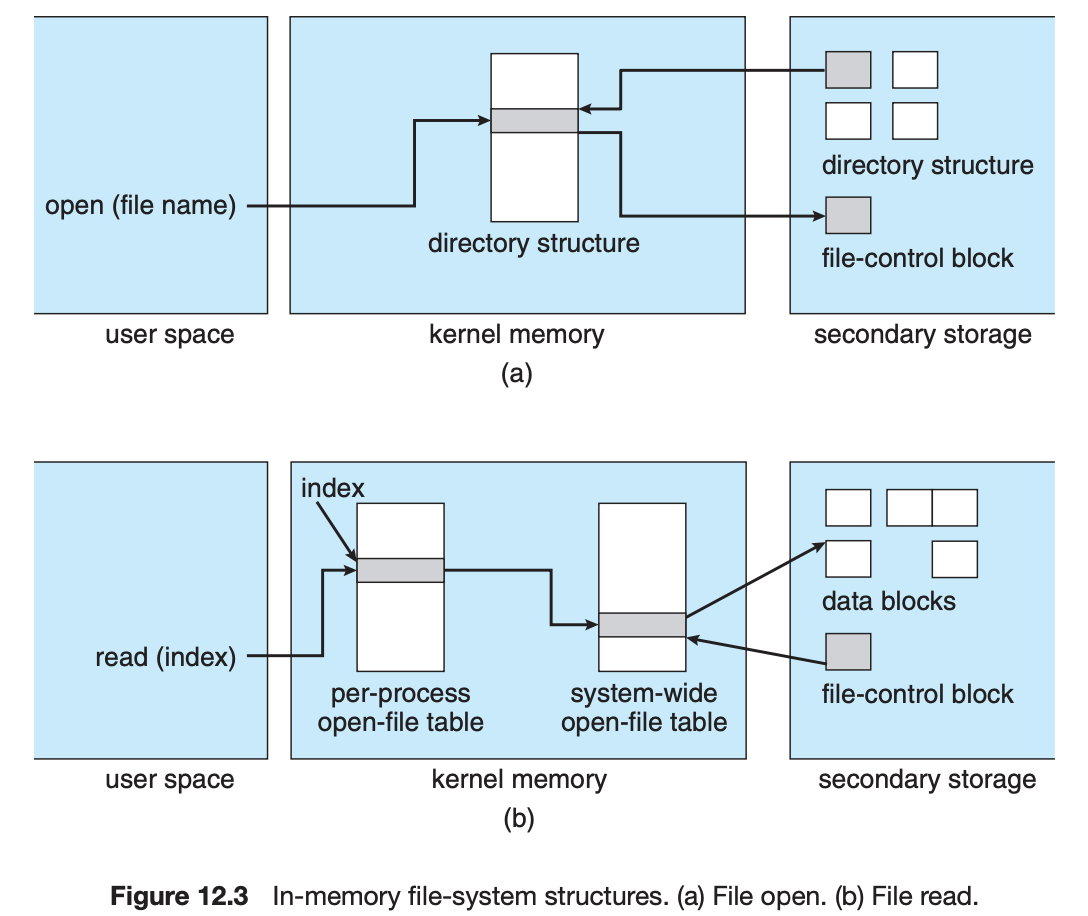
\includegraphics[scale=0.5]{37.png}    
\caption{File Open and File Read}
\end{center}
\end{figure}

To create a new file, an application program calls the logical file system. The logical file system knows the format of the directory structures. To create a new file, it allocates a new FCB. Then, the system reads the appropriate directory into memory, updates it with the new file name and FCB, and writes it back to the disk. Now that a file has been created, it can be used for I/O.

\subsubsection{Directory Implementation}
\begin{itemize}
    \item \textbf{Linear List}: The simplest way to implement a directory is to use a linear list of file names with pointers to data blocks. To create a new file, we must first search the directory to make sure that there are no existing files with the same name. Then, add a new entry to the end of the directory. To delete a file, search for the named file in the directory, and then release the allocated space. However, the disadvantage of a linear list is that \textit{we need a linear search to find the file}. Therefore, this method is simple to program but time-consuming to execute. Directory information is used frequently, and users may notice when access is slow. In fact, many operating systems implement a software cache that stores the most recently used directory information. A cache hit does not require a constant re-reading of information from disk.
    \item \textbf{Hash Table}: Another data structure is hash tables. In this method, linear list stores directory entries, but a hash data structure is also used. The hash table takes the calculated value from the file name and returns a pointer to the file name in the linear list. This can significantly reduce directory browsing time. The main difficulty is usually a fixed size and the dependency of the hash function on that size. For example, if an existing hash table is full and we want to create a new file, we need to increase the size of the hash table, a new hash function that needs to remap the file names accordingly, and reconfigure the existing directory entries to reflect the new hash function values.
\end{itemize}

\subsubsection{Hard Disk Structure}
\begin{figure}[h]
\begin{center}
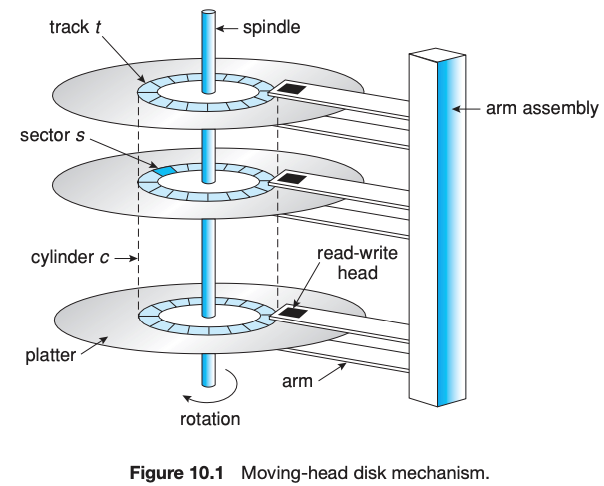
\includegraphics[scale=0.7]{38.png}    
\caption{Inside the Hard Disk}
\end{center}
\end{figure}

\begin{itemize}
    \item \textbf{Platter}: It is a magnetic disc that records actual data. There are multiple platters as shown in the figure, and they can be used back and forth. A platter consists of multiple tracks.
    \item \textbf{Track}: It is a region that forms a concentric circle of the platter.
    \item \textbf{Sector}: The area where a track is divided into several is called a sector. The sector size is typically 512 bytes, and it is usually used in groups.
    \item \textbf{Cylinder}: A cylinder is the set of the same track positions in all platters.
\end{itemize}

Earlier, it was said that sector is used in groups, which is called a block. Hard disks are also called block devices because they read and write in blocks. A simple way to check that your hard disk is reading and writing block by block is to write down the alphabet ‘a’ in a notepad program and save it. ‘a’ has a size of 1 byte as a character, and if you check the properties of the actual saved text file, you can see that 4KB (one block size) is allocated to the disk. (The actual disk allocation size varies by operating system. The following tests were performed in a MacBook OS environment.) Therefore, a disk can be seen as a collection of empty blocks. So \textit{how does the operating system allocate a free block for each file?}

\begin{figure}[h]
\begin{center}
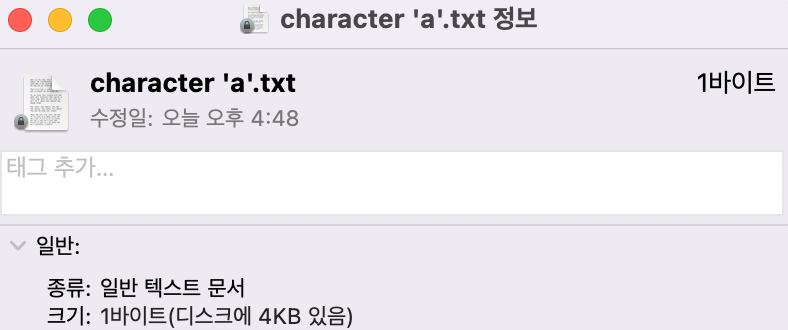
\includegraphics[scale=0.7]{39.png}    
\caption{Example File}
\end{center}
\end{figure}

\subsubsection{Allocation Methods}
In almost every case, many files are stored on the same disk. The main problem is how to allocate space for these files so that they can effectively utilize disk space and access files quickly. The three main ways to allocate disk space are popular: continuous, linked, and indexed.

• \textit{Contiguous Allocation}: Continuous allocation is literally allocating a file in contiguous blocks. The advantage of continuous allocation is that the movement of the disk header can be minimized, thereby increasing I/O performance. This method is used by IBM in the past, and is mainly suitable for video, music, VOD, etc.
 Contiguous allocation is stored sequentially, so the operating system can access the desired block directly with the starting block number obtained from the directory. However, this method has major drawbacks and is rarely used today. When allocating and erasing files repeatedly, there is an empty space (hole) in the middle, and since continuous allocation must find contiguous space, external fragmentation problems occur. External fragmentation results in a very high waste of disk space. Another problem is that the actual size is unknown when saving the file. In particular, files that are used continuously can continue to grow in size, so it is very inappropriate to allocate them continuously. 

• \textit{Linked Allocation}: With linked allocation, each file is a list of disk blocks and the disk blocks can be scattered anywhere on the disk. To create a new file, select any empty block as the first block, and if the file grows, we only need to assign another block and link it to the existing block. Linked allocation can be assigned regardless of location, so there is no external fragmentation problem (= no disk waste).
However, there are also various problems with linked allocation:

\begin{itemize}
    \item Sequential access is possible, but direct access is \textbf{not}. Because the blocks of the file are all scattered, so we cannot directly access the block at the desired location with the starting block number.
    \item More than 4 bytes of damage is caused to store the pointer.
    \item \textit{Low reliability}: if the pointer of the middle block breaks, all subsequent blocks are not accessible.
    \item \textit{Slow speed}: Since the blocks are all scattered, there is just as much movement of the disk header.
\end{itemize}

One of the improvements to the above problems is the FAT (File Allocation Table) system, which is the same connection allocation method. The FAT system collects only the pointers to the next block, creates a table, and stores it in one block.

\begin{figure}[h]
\begin{center}
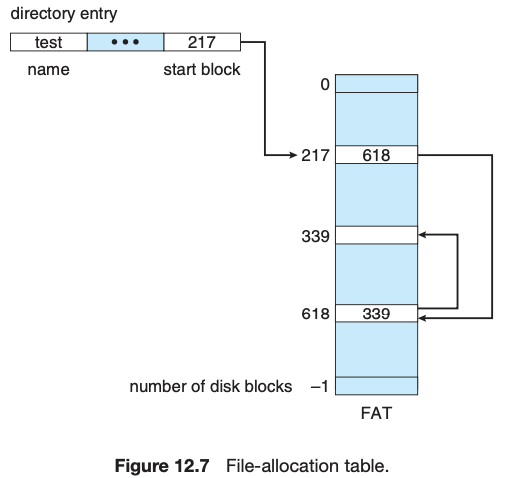
\includegraphics[scale=0.7]{40.png}    
\caption{FAT System Table}
\end{center}
\end{figure}

If we look at the FAT stored in block 0, the index of the table is the block number of the entire disk, and \textit{each index stores the next block number}. The table entry in the last block has a special value (-1) indicating the end of the file.

• Indexed Allocation: Index allocation, like connection allocation, assigns data to random block numbers, but stores the allocated block pointers separately in a block. These blocks are called index blocks, and there is one index block per file. Index allocation differs from other allocations in directory information, which stores the index block number rather than the starting block number.

Index allocation can be accessed directly and since there is no need to allocate continuously, there is no external fragmentation problem. Index allocation is primarily used by Unix/Linux. The disadvantage of index allocation is that even small files use one block as an index block, so storage space is lost. And we can't store a large file with a single index block. Let's take a look at the combined scheme that Unix uses to solve this.

\begin{figure}[h]
\begin{center}
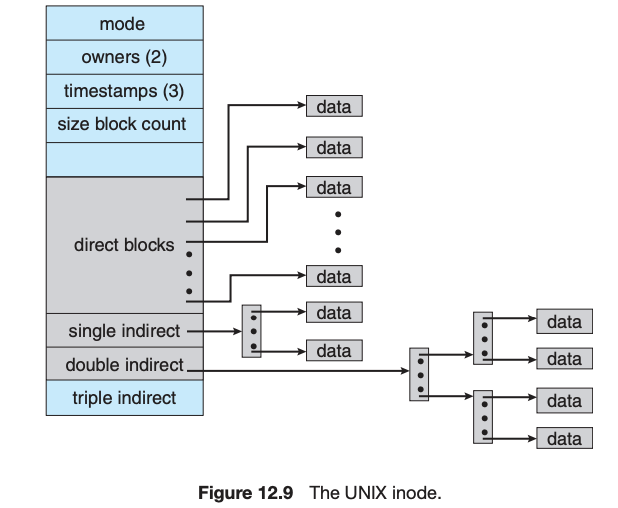
\includegraphics[scale=0.7]{41.png}    
\caption{UNIX Inode}
\end{center}
\end{figure}

It keeps the first 15 pointers of the index block at the index of the file, and the first 12 pointers point to the direct block. The direct block has the address of the block containing the data of the file. Therefore, there is no need for an index block for data in small files that do not exceed 12 blocks. And the next three pointers point to indirect blocks. The three pointers point to a single indirect block, a double indirect block, and a triple indirect block, respectively, which is an index block that stores the address of the block rather than the block that stores the data.

\subsection{References}
For some figures, we borrowed figures from Avraham Silberschatz, Operating System Concepts \nth{10} edition. The copyrights of each figures belongs to their respective authors.

\pagebreak

\section{Compiling and Building} 
There are 1 directory in this \texttt{git}.
\begin{itemize}
   \item \texttt{MyFS}: Simple file system implementation
\end{itemize}

\texttt{MyFS} supports both \texttt{CMake} and \texttt{Makefile}. By using the \texttt{Makefile}, you can compile the project. \texttt{Makefile} includes following optional recipes:
\begin{itemize}
   \item \texttt{clean}: For cleaning up object files and compiled program.
   \item \texttt{debug}: For debugging purpose. This will enable \texttt{-DDEBUG} option. 
\end{itemize}

For example, if you were to compile and build \texttt{MyFS}, you can do it so by following command:
\\
\begin{center}
\begin{code}
\begin{minted}[frame=single,framesep=10pt]{bash}
$ cd ./MyFS
$ make 
\end{minted}
\captionof{listing}{Using \texttt{Makefile} for compiling MyFS}
\end{code}
\end{center}

This will automatically build project and generate an executable file named \texttt{MyFS}. If you would like to use \texttt{CMake} instead, you can do it so by following commands:
\\
\begin{center}
\begin{code}
\begin{minted}[frame=single,framesep=10pt]{bash}
$ cd ./MyFS
$ mkdir build & cd build
$ cmake .. & make .
\end{minted}
\captionof{listing}{Using \texttt{CMake} for compiling MyFS}
\end{code}
\end{center}

\warningbox{Please place at least one valid \texttt{.img} file in the same directory as \texttt{MyFS} executable. Otherwise, the program will consider that there is no disk images and will quit execution right away. For the best practice, please place \texttt{disk.img} that professor offered us in the same directory as \texttt{MyFS}. No other \texttt{.img}s were checked working.}
For executing \texttt{MyFS} you can do it so by following command:
\\

\begin{center}
\begin{code}
\begin{minted}[frame=single,framesep=10pt]{bash}
$ ./MyFS
...
            Simple File System Simulator
[INFO] Successfully mounted disk 0: disk.img
MyFS@root >>
\end{minted}
\captionof{listing}{Executing \texttt{MyFS}}
\end{code}
\end{center}

Each commands will be explained in later pages.
\pagebreak

\section{Design and Sketch}
\subsection{Choosing Topic}
There were too many choices for this project. Meaning that not only we were allowed to chose project 2 or project 3, we also had choice of implementing project 3 in our way. So, the fundamental reason that we chose project 3 over project 3 was the fact that it is more 'realistic' than the virtual memory. That is, virtual memory implementation will live in a virtual world that is quite different from our real computers. Of course, we could have implemented page tables, swapping, dynamic address, shared memory and etc. However those things were not that much interesting compared to our own file system in terms of 'realism'. However, with file system implementation, we can kind of mimic OS operations and can literally store and read data into our own file system. Therefore we chose project 3 over project 2. 


Within project 3, there were also lots of choices that we can make. Since in class we talked about file system after virtual memory, project 3 was kind of running short on time. There were some brilliant ideas on project 3, however was not able to implement due to time being:
\begin{itemize}
    \item \textbf{Scheduling}: Since we have implemented a scheduling simulation in project 1, we were thinking of combining our file system into the program. Since the scheduling were performing CPU burst and IO burst sequentially, we thought of implementing the IO burst into our own file system. 
    \item \textbf{RAID 0}: In our mid term exam, the last question was about having a single file across many disks. That kind of gave us the inspiration and motivation for making a simple RAID system with RAID 0. Implementing a real RAID 0 system would have been a tough subject, however implementing a simple strafing have seemed to be feasible. Also, we were planning to make some comparisons about reading and writing operations to one disk versus reading and writing operations to multiple RAID 0 disks.
    \item \textbf{RAID 3 and 4}: As we have mentioned before, RAID seemed to be a good topic. Also since we were thinking about implementing strafing, we also wanted to implement parity checking in a single disk. We also planned to have some comparison between RAID and non raid disks in terms of failure and data loss as well. 
\end{itemize}
Those three subjects seemed to be very interesting. However, since we were running short on time, we had select a topic that we can implement in time for sure. Therefore those three subjects were not selected. This does not mean those 3 topics were discarded forever. We will be implementing those topics if we have some free time in the future. After lots of consideration, we came to conclusion that we would like to make a simple file system that works like \texttt{bash}. Therefore, we decided to make a simple (so called) terminal that can interact between user and perform disk operations: \textit{write, read, move, copy and etc}. 

\subsection{Requirements}
In order for us to implement those features, we need to have some basic bootstrapping on disk file system as well as implementing advanced features. The basic features that we must implement were as it follows:
\begin{itemize}
    \item \textbf{Mounting disk}: In order for us to use a disk, we need to mount it. This sounds easy, however needs some internal operations. Those operations require: reading superblock, reading inode table.
    \item \textbf{Directory}: For our program to correctly print out the files and its contents, we need to implement directory. Also the directory must indicate a specific inode that a specific directory entry is using.
    \item \textbf{File}: Including directory, we need to make our program read and write into specific disk blocks in order to read contents from a specific file. The actions that were required were: read, write, append.
\end{itemize}
Those three elements were the very basic elements that were required. On top of those basic requirements, we wanted to put more advanced features. Those were:

\begin{itemize}
    \item \textbf{Directory Navigation}: We need to make our program traverse throughout the directories in the file system just like Linux environments. For example, we wanted \texttt{cd} command from Linux.
    \item \textbf{Creation}: The program needed to create a new empty file when user requested. This requires assigning empty inode and assigning empty blocks. We wanted \texttt{touch} and \textttt{mkdir} command from Linux.
    \item \textbf{Deletion}: Since we have feature of creating a new file, we also needed to have deletion features. Not only just deleting a single regular file, we also wanted to implement recursive file deletion when deleting a directory. That is, we wanted \texttt{rm} and \texttt{rm -rf}.
    \item \textbf{Read}: Since basic requirements supported file reading, we wanted to implement a simple interface for file open and read combined. That is, we wanted to mimic \texttt{cat} command from Linux.
    \item \textbf{Write and Appending}: Writing into a file and appending into a file is necessary as well. We wanted a simple interface that supports easy writing and easy reading that internally performs file open and write (or append). This was to mimic \texttt{echo "foo" > bar.txt} or \texttt{echo "foo" >> bar.txt}. 
    \item \textbf{Copy}: Modern file system supports copying file. Of course, we could have just copied a duplicate file. However, since our program runs in a small disk, creating a new file whenever a file was being copied was not a good idea. Therefore, we wanted "\textbf{Copy on Write}" action implemented into our program.
    \item \textbf{Permissions}: Linux offers some file permissions. We also wanted to implement the feature of file permission editing just like \texttt{chmod}. We also considered about having multiple users and making each user have some permissions as well. (The multiple user part was not implemented due to the time being)
    \item \textbf{Move and Rename}: Just like Linux, we wanted to make our program rename a file or directory when user requested. Also we wanted to make files 'movable'. This was intended to mimic \textttt{mv} command in Linux.
    \item \textbf{Stats and Listing}: In order for us to get information on each files and directories, we needed something like \texttt{stat} and \texttt{ls}. Those were implemented as well.
    \item \textbf{Caching}: This is not 100\% caching, however the intention was to have the directory structure cached in the memory. By this, we wanted to make our program access to a file faster.
\end{itemize}

\subsection{Designing Directory}
The most important thing that we needed to implement was the directory structure. There are lots of ways to implement directory structures. However, the one that we chose to implement our directory structure was "\textbf{Left Child Right Sibling}" tree. The reason of choosing left child right sibling tree for storing directory structure was that this the fact that it very easy for modification. In file system, we need some operations that remove link from a single entry, such as delete and move. Also we need some operations that add links to the entire directory structure, such as creation and move. Therefore, due to ease of modifying the tree structure, we selected left child right sibling tree for storing our directory structure. Let's assume that we have following directory stored in our file system:

\begin{figure}[h]
\begin{center}
\begin{minipage}{7cm}
\dirtree{%
.1 /.
.2 foo.
.2 bar.
.3 baz.
.3 qux.
.2 quux.
}
\end{minipage}
\end{center}
\caption{Example file system structure}
\end{figure}

As its name indicates, child element goes into the left side of the node. The for siblings, the node goes into the left side. With the directory structure, we can make following understanding:
\begin{itemize}
    \item \texttt{/} has child \texttt{foo}, but has no sibling
    \item \texttt{foo} has no child, but has a sibling \texttt{bar}
    \item \texttt{bar} has a child \texttt{baz}, and also has a sibling \texttt{quux}
    \item \texttt{baz} has no child, but has a sibling \texttt{qux}.
    \item \texttt{quux} has no child and no sibling.
\end{itemize}


With left child right sibling tree, the structure will be represented as following tree:

\begin{figure}[h]
\begin{center}
\begin{forest}
  [/
     [foo
       [NULL]
       [bar
        [baz
         [NULL]
         [qux]
        ]
        [quux]
       ]
     ]
    [NULL
    ]
  ]
\end{forest}
\end{center}
\caption{Example Left Child Right Sibling Tree}
\end{figure}
Please be aware that for leaf nodes, the sibling and child is not denoted. .Huge thanks to \texttt{forest} and \texttt{tikz} for this simple yet beautiful tree. Now, let's suppose that we wanted to delete \texttt{/bar/baz} from the directory, the tree will be transformed into the following tree:
\begin{figure}[h]
\begin{center}
\begin{forest}
  [/
     [foo
       [NULL]
       [bar
        [qux]
        [quux]
       ]
     ]
    [NULL
    ]
  ]
\end{forest}
\end{center}
\caption{Deleted \texttt{/bar/baz}}
\end{figure}
Now let's suppose that we would like to create a file \texttt{/corge}. Then the tree will become something like below:
\begin{figure}[h]
\begin{center}
\begin{forest}
  [/
     [foo
       [NULL]
       [bar
        [qux]
        [quux
        [NULL]
        [corge]
        ]
       ]
     ]
    [NULL
    ]
  ]
\end{forest}
\end{center}
\caption{Created \texttt{/corge}}
\end{figure}

As you can see, this tree is very easy to modify as well as easy to maintain. As we all know, implementing a tree structure in \texttt{C} is also easy with a little help of \texttt{pointer} operations. We made a \texttt{struct} data type named \texttt{entry_t} that will help us represent the tree. \texttt{struct entry_t} is defined in \texttt{disktree.h}.
\\
\begin{center}
\begin{code}
\begin{minted}[frame=single,framesep=10pt]{c}
struct entry_t {
    char name[16];
    unsigned int disk_index;
    unsigned int inode_index;
    struct entry_t *sibling;
    struct entry_t *child;
    struct entry_t *parent;
};
\end{minted}
\captionof{listing}{Definition of \texttt{struct entry_t}}
\end{code}
\end{center}
For easy operations in the future, such as \texttt{cd ..} and \texttt{mv ..}, there is extra field that points to the parent element. With \texttt{struct entry_t}, the pseudo-code for adding an entry into a directory tree will be like below:

\begin{algorithm}
\caption{Adding Entry to Directory}\label{alg:cap}
\begin{algorithmic}
    \Procedure{Insert}{$new, directory$}
    \If{$directory.child = NULL$} \Comment{The directory was empty}
        \State $directory.child \gets new$
    \Else
        \State $peer \gets directory.child$
        \While{$peer.sibling \neq NULL$} \Comment{Find the last sibling}
            \State $peer \gets peer.sibling$
        \EndWhile
        \State $peer.sibling \gets new$ \Comment{Add sibling to last sibling}
    \EndIf
\end{algorithmic}
\end{algorithm}
The pseudo-code will insert a new entry into the directory. Since the algorithm needs to find the last sibling, the time complexity will become $O(n)$ if there are $n$ entries in the target directory. Yes, there will be a better solution with better time complexity, however the best we can think of is this one until now. Since we have checked inserting a new entry into a directory, let's check removing an entry from the directory. The pseudo-code will become something like below:

\begin{algorithm}
\begin{algorithmic}
    \Procedure{Remove}{$target, directory$}
        \State $peer \gets directory.child$
        \While{$peer.sibling \neq NULL$} \Comment{Find sibling connected to target}
            \If {$peer.sibling = target$}
                \State Break loop
            \EndIf
            \State $peer \gets peer.sibling$
        \EndWhile
        \State $peer.sibling \gets target.sibling$ \Comment{Un-link target}
\end{algorithmic}
\end{algorithm}

The pseudo-code will remove entry from the directory if found. For simple explanation, this pseudo-code assumes that the file exists in the directory. This also is an $O(n)$ operation when there is $n$ entries in the target directory. In real implementations, to avoid \texttt{SIGSEV}, there are some protection measures added as well.

Those two pseudo-codes were implemented under various functions in \texttt{diskutil.c}. To name a few functions that are using this pseudo-code, the following list are the functions:
\begin{itemize}
    \item \texttt{create_file}:  When creating a new file.
    \item \texttt{delete_file}: When deleting a file.
    \item \texttt{r_delete_directory}: When deleting a directory.
    \item \texttt{copy_file}: When copying a file.
    \item \texttt{handle_cow}: When \textit{Copy on Write} was triggered.
    \item \texttt{move_file}: When moving a file.
\end{itemize}
\pagebreak
\section{Implementation and Usage}
Since there are lots of features implemented in this program, we decided to introduce each implementations and usages at the same time. This program offers a list of commands and each commands were designed to mimic actions from the original commands in Linux. Those commands are as it follows:

\begin{center}
\begin{table}[h]
\begin{tabularx}{1.0\textwidth} { 
  | >{\centering\arraybackslash}X 
  | >{\centering\arraybackslash}X 
  | >{\centering\arraybackslash}X | }
 \hline
 \textbf{Command} & \textbf{Description} & \textbf{Original Linux Command}\\
 \hline
 \texttt{ls} & Lists element in this directory & \texttt{ls}\\
  \hline
 \texttt{cat} & Shows file content & \texttt{cat}\\
  \hline
 \texttt{chmod} & Changes file permission & \texttt{chmod}\\
  \hline
 \texttt{stat} & Shows file stats & \texttt{stat}\\
  \hline
 \texttt{touch} & Creates empty file & \texttt{touch}\\
  \hline
 \texttt{mkdir} & Creates empty directory & \texttt{mkdir}\\
   \hline
 \texttt{rm} & Removes a file & \texttt{rm}\\
    \hline
 \texttt{rmdir} & Removes a directory recursively & \texttt{rm -rf}\\
    \hline
 \texttt{vstat} & Prints out volume stats & N/A\\
    \hline
 \texttt{write} & Writes data to file & \texttt{echo "foo" > bar}\\
    \hline
 \texttt{append} & Appends data to file & \texttt{echo "foo" >> bar}\\
    \hline
 \texttt{cd} & Changes current working directory & \texttt{cd}\\
    \hline
 \texttt{cp} & Copies a file & \texttt{cp}\\
    \hline
 \texttt{rename} & Renames a file or directory & \texttt{mv}\\
    \hline
 \texttt{mv} & Moves a file into other directory & \texttt{mv}\\
    \hline
 \texttt{cwd} & Prints current working directory & \texttt{cwd}\\
    \hline
 \texttt{xmas} & Prints Christmas tree & N/A \\
    \hline
 \texttt{cxmas} & Prints Christmas tree in color & N/A \\
    \hline
\end{tabularx}
\caption{Table of Implemented Commands}
\end{table}
\end{center}

All commands were confirmed it working on a private server with following environments:
\begin{itemize}
    \item \textbf{OS}: Ubuntu 22.04 LTS
    \item \textbf{CPU}: Intel(R) Core(TM) i9-7940X CPU @ 3.10GHz
    \item \textbf{RAM}: 32GB
    \item \textbf{Endian}: \underline\textbf{Little Endian}
\end{itemize}
Also, the program was checked it working with the disk image \texttt{disk.img} that professor gave us. With other \texttt{.img} files, this program was not checked it working.
\pagebreak

\subsection{\texttt{ls}}
\subsubsection{Feature}
This command prints out all the entries in current working directory.
\subsubsection{Usage}
\begin{center}
\texttt{ls <args>}
\end{center}
This program offers following arguments
\begin{itemize}
    \item \texttt{-al}: Shows permission, file size and name of all files.
    \item \texttt{-ald}: Shows detailed stats of each files, including inode and disk information
\end{itemize}

\subsubsection{Example Outputs}
\par
With default \texttt{ls}, it will show entries and its names like following:
\\
\begin{center}
\begin{code}
\begin{minted}[frame=single,framesep=10pt]{bash}
MyFS@root >> ls
file_1  file_2  file_3  file_4  file_5  file_6  file_7  file_8  file_9  ...
file_72  file_73  file_74  file_75  file_76  file_77  file_78  file_79  ...
file_82  file_83  file_84  file_85  file_86  file_87  file_88  file_89  ...
file_92  file_93  file_94  file_95  file_96  file_97  file_98  file_99  ...
\end{minted}
\end{code}
\end{center}
With \texttt{ls -al}, it will show entries and its names with permission and size like following:
\\
\begin{center}
\begin{code}
\begin{minted}[frame=single,framesep=10pt]{bash}
MyFS@root >> ls -al
-rwxrwxrwx         37 file_1
-rwxrwxrwx         40 file_2
...
-rwxrwxrwx         38 file_99
-rwxrwxrwx         42 file_100
\end{minted}
\end{code}
\end{center}
With \texttt{ls -ald}, it will show inode information and disk index of each files like following:
\\
\begin{center}
\begin{code}
\begin{minted}[frame=single,framesep=10pt]{bash}
MyFS@root >> ls -ald
-rwxrwxrwx         37 file_1(Inode 3 @ disk 0)
-rwxrwxrwx         40 file_2(Inode 4 @ disk 0)
...
-rwxrwxrwx         38 file_99(Inode 101 @ disk 0)
-rwxrwxrwx         42 file_100(Inode 102 @ disk 0)
MyFS@root >>
\end{minted}
\end{code}
\end{center}
\pagebreak
\subsubsection{Implementation}
This was implemented by traversing all the siblings of current directory. The pseudo code is like below:
\begin{algorithm}
\caption{Directory Listing}\label{alg:cap}
\begin{algorithmic}
    \Procedure{ls}{$directory$}
    \If{$directory.child = NULL$} \Comment{The directory was empty}
        \State Return
    \Else
        \State $peer \gets directory.child$
        \While{$peer.sibling \neq NULL$} \Comment{Print all names of entries}
            \State Print $peer.sibling.name$
            \State $peer \gets peer.sibling$
        \EndWhile
    \EndIf
\end{algorithmic}
\end{algorithm}

The command is implemented with following functions:
\begin{itemize}
    \item \texttt{ls}: Under \texttt{ui.c} for wrapping \texttt{impl_ls}
    \item \texttt{impl_ls}: Under \texttt{diskutil.c} for printing out all the entries.
\end{itemize}

\subsubsection{ETC}
By default, this program sets a line break in every 10 elements. If you would like to how more files in a single line, you can modify the length by defined as \texttt{LS_SPLIT_COUNT} under \texttt{diskutil.h}.
\pagebreak

\subsection{\texttt{cat}}
\subsubsection{Feature}
\warningbox{This command will not read data from a directory file}
This command prints out the content in a file. 
\subsubsection{Usage}
\begin{center}
\texttt{cat [file]}
\end{center}

\subsubsection{Example Outputs}
When executing \texttt{cat} to a single file it will be shown like following:
\\
\begin{center}
\begin{code}
\begin{minted}[frame=single,framesep=10pt]{bash}
MyFS@root >> cat file_1
file 1 741474268 913453413 395175819
\end{minted}
\end{code}
\end{center}
When executing \texttt{cat} to a directory file it will be shown like following:
\\
\begin{center}
\begin{code}
\begin{minted}[frame=single,framesep=10pt]{bash}
MyFS@root >> cat directory
cat: directory: is a directory
\end{minted}
\end{code}
\end{center}
When executing \texttt{cat} to a non-existing file it will be shown like following:
\\
\begin{center}
\begin{code}
\begin{minted}[frame=single,framesep=10pt]{bash}
MyFS@root >> cat unknown
cat: unknown: No such file or directory
\end{minted}
\end{code}
\end{center}

\subsubsection{Implementation}
When this command is called, following operations are held in sequence:
\begin{enumerate}
    \item Open file in \texttt{R} mode and lock file.
    \item Retrieve block information from inode.
    \item Read block information and store it to buffer.
    \item Close file and unlock file, then print it out.
\end{enumerate}

The command is implemented with following functions:
\begin{itemize}
    \item \texttt{cat}: Under \texttt{ui.c} for wrapping \texttt{impl_cat}
    \item \texttt{impl_cat}: Under \texttt{diskutil.c} for opening and requesting read then printing buffer.
    \item \texttt{read_file_data}: Under \texttt{diskutil.c} for reading actual data from disk in binary then storing it to buffer.
\end{itemize}
\pagebreak

\subsection{\texttt{chmod}}
\subsubsection{Feature}
This command changes permission of a file, including a directory file.
\subsubsection{Usage}
\begin{center}
\texttt{chmod [permission] [file]}
\end{center}
For permission, this command uses the same permission as the Linux uses. Consider a example like below:
\begin{itemize}
    \item User has all \texttt{RWX} permission.
    \item Group has only \texttt{R} permission.
    \item Others have only \texttt{R} permission.
\end{itemize}

This will make permission as following:
\begin{center}
\begin{table}[h]
\begin{tabularx}{1.0\textwidth} { 
  | >{\centering\arraybackslash}X 
  | >{\centering\arraybackslash}X 
  | >{\centering\arraybackslash}X 
  | >{\centering\arraybackslash}X | }
 \hline
  \textbf{Target} & \textbf{R} & \textbf{W} & \textbf{X}\\
  \hline
   User & 1 & 1 & 1 \\
     \hline
   Group & 1 & 0 & 0 \\
     \hline
   Others & 1 & 0 & 0 \\
    \hline
\end{tabularx}
\caption{Example Permission}
\end{table}
\end{center}

Therefore, this will make the total permission as \texttt{744}. So, example execution will be \texttt{chmod 744 foo}.
\subsubsection{Example Outputs}
When executing \texttt{chmod} to a file named \texttt{foo} with original permission of \texttt{777} and changing it to \texttt{744}:
\\
\begin{center}
\begin{code}
\begin{minted}[frame=single,framesep=10pt]{bash}
MyFS@root >> stat foo
   File: foo    Empty file: 1
   Size: 3    IO Block: 1
   Disk: disk.img (0)    Inode: 104
   Access: (0777/-rwxrwxrwx)
MyFS@root >> chmod 744 foo
MyFS@root >> stat foo
   File: foo    Empty file: 1
   Size: 3    IO Block: 1
   Disk: disk.img (0)    Inode: 104
   Access: (0744/-rwxr--r--)
\end{minted}
\end{code}
\end{center}

\pagebreak
When executing \texttt{chmod} with invalid permission \texttt{999}
\\
\begin{center}
\begin{code}
\begin{minted}[frame=single,framesep=10pt]{bash}
MyFS@root >> chmod 999 foo
chmod: invalid mode: ‘999’
\end{minted}
\end{code}
\end{center}
When executing \texttt{chmod} to an unknown file.
\\
\begin{center}
\begin{code}
\begin{minted}[frame=single,framesep=10pt]{bash}
MyFS@root >> chmod 777 bar
chmod: cannot access 'bar': No such file or directory
\end{minted}
\captionof{listing}{Example Execution of \texttt{cat} Unknown File}
\end{code}
\end{center}

\subsubsection{Implementation}
When this command is called, following operations are held in sequence:
\begin{enumerate}
    \item Lock file and check if copy on write is required.
    \item Retrieve inode from \texttt{struct entry_t}.
    \item Change permission to the designated one.
    \item Write inode back to the disk.
    \item Unlock file
\end{enumerate}

The command is implemented with following functions:
\begin{itemize}
    \item \texttt{chmod}: Under \texttt{ui.c} for wrapping \texttt{impl_chmod}
    \item \texttt{impl_cat}: Under \texttt{diskutil.c} for finding inode from \texttt{struct entry_t} and changing the information then writing back to the disk.
\end{itemize}

\subsubsection{}{ETC}
This program modified the definitions of file permissions defined in \texttt{fs.h} that professor gave us. For ease of use and for better permission control, we have changed values like following:

\begin{center}
\begin{table}[h]
\begin{tabularx}{1.0\textwidth} { 
  | >{\centering\arraybackslash}X 
  | >{\centering\arraybackslash}X 
  | >{\centering\arraybackslash}X | }
 \hline
   MACRO & Original & New \\
     \hline
   \texttt{INODE_MODE_AC_USER_R} & 0x001	& 0x400 \\
    \hline
   \texttt{INODE_MODE_AC_USER_W} & 0x002	& 0x200 \\
    \hline
   \texttt{INODE_MODE_AC_USER_X} & 0x004	& 0x100 \\
    \hline
   \texttt{INODE_MODE_AC_OTHER_R} & 0x010	& 0x004 \\
    \hline
   \texttt{INODE_MODE_AC_OTHER_W} & 0x020	& 0x002 \\
    \hline
   \texttt{INODE_MODE_AC_OTHER_X} & 0x040	& 0x001 \\
    \hline
   \texttt{INODE_MODE_AC_GRP_R} & 0x100	& 0x040 \\
    \hline
   \texttt{INODE_MODE_AC_GRP_W} & 0x200	& 0x020 \\
    \hline
   \texttt{INODE_MODE_AC_GRP_X} & 0x400	& 0x010 \\
    \hline
    
\end{tabularx}
\caption{Example Permission}
\end{table}
\end{center}

\subsection{\texttt{stat}}
\subsubsection{Feature}
This command prints the statistics in a file
\subsubsection{Usage}
\begin{center}
\texttt{stat [file]}
\end{center}

\subsubsection{Example Outputs}
If we had a file that is an original file without any indirection to other inode, this will be shown:
\\
\begin{center}
\begin{code}
\begin{minted}[frame=single,framesep=10pt]{bash}
MyFS@root >> stat file_1
   File: file_1    Empty file: 0
   Size: 37    IO Block: 1
   Disk: disk.img (0)    Inode: 3
   Access: (0777/-rwxrwxrwx)
   Indirection(s) from: 105,
\end{minted}
\end{code}
\end{center}

If we were performing \texttt{stat} to a copied file, this will be shown. In this case \texttt{copied} was a file copied from \texttt{file_1} and was not triggered copy on write operation 
 yet, this will be shown:
\\
\begin{center}
\begin{code}
\begin{minted}[frame=single,framesep=10pt]{bash}
MyFS@root >> stat copied
   File: copied    Empty file: 0
   Size: 37    IO Block: 1
   Disk: disk.img (0)    Inode: 105
   Access: (0777/-rwxrwxrwx)
   Indirection to: 3
\end{minted}
\end{code}
\end{center}


\subsubsection{Implementation}
When this command is called, following operations are held in sequence:
\begin{enumerate}
    \item Retrieve inode from \texttt{struct entry_t}.
    \item Check in-going and out-going indirection for this inode.
    \item Print out the information.
\end{enumerate}

The command is implemented with following functions:
\begin{itemize}
    \item \texttt{stat}: Under \texttt{ui.c} for wrapping \texttt{impl_stat}
    \item \texttt{impl_stat}: Under \texttt{diskutil.c} for reading and printing out the inode information.
\end{itemize}
\pagebreak

\subsection{\texttt{touch}}
\subsubsection{Feature}
This command creates an empty regular file.
\subsubsection{Usage}
\begin{center}
\texttt{touch [file]}
\end{center}

\subsubsection{Example Outputs}
We wanted to create a file named new, then \texttt{cat} the new file:
\\
\begin{center}
\begin{code}
\begin{minted}[frame=single,framesep=10pt]{bash}
MyFS@root >> touch new
MyFS@root >> ls
...
...  file_95  file_96  file_97  file_98  file_99  file_100  new
MyFS@root >> cat new

MyFS@root >>
\end{minted}
\end{code}
\end{center}

\subsubsection{Implementation}
When this command is called, following operations are held in sequence:
\begin{enumerate}
    \item Allocate an empty inode. Initial size is 3bytes for marking that this inode is assigned. Also, the initial permission is set to \texttt{777}.
    \item Allocate an empty block and set first bit to \texttt{\n}.
    \item Write inode and empty block to the disk.
    \item Update entry in the left child right sibling tree.
\end{enumerate}

The command is implemented with following functions:
\begin{itemize}
    \item \texttt{touch}: Under \texttt{ui.c} for wrapping \texttt{impl_touch}.
    \item \texttt{impl_touch}: Under \texttt{diskutil.c} for creating an empty regular file.
    \item \texttt{create_file}: Under \texttt{diskutil.c} for actually creating an empty file. This function allocates free inode and free data blocks as well.
    \item \texttt{dir_add_child}: Under \texttt{diskutil.c} for adding an child element to parent directory.
\end{itemize}

\warningbox{This program does not manage fragmentation. That is, if the new file acquired disk block number 3, and the next block 4 was already allocated, this will get fragmented. The program does not take care of fragmentation and has no way of relaxing fragmentation. Also, the initial size of the file is set to 3 bytes to mark free inode vector that this one is assigned and is not ready to be used. Therefore, the actual byte written on the disk and the size that inode indicates will differ initially.}

\pagebreak

\subsection{\texttt{mkdir}}
\subsubsection{Feature}
This command creates an empty directory file.
\subsubsection{Usage}
\begin{center}
\texttt{mkdir [file]}
\end{center}

\subsubsection{Example Outputs}
We wanted to create a directory named new\_dir, then \texttt{cd} into the new directory:
\\
\begin{center}
\begin{code}
\begin{minted}[frame=single,framesep=10pt]{bash}
MyFS@root >> mkdir new_dir
MyFS@root >> ls
...
...  file_95  file_96  file_97  file_98  file_99  file_100  new_dir
MyFS@root >> cd new_dir
MyFS@root/new_dir >> ls

MyFS@root/new_dir >>
\end{minted}
\end{code}
\end{center}

\subsubsection{Implementation}
When this command is called, following operations are held in sequence:
\begin{enumerate}
    \item Allocate an empty inode. Initial size is 20bytes for marking that this inode is assigned. Also, the initial permission is set to \texttt{777}.
    \item Allocate an empty block and set two disk entries. Those are \texttt{.} and \texttt{..}.
    \item Write inode and empty block to the disk.
    \item Update entry in the left child right sibling tree.
\end{enumerate}

The command is implemented with following functions:
\begin{itemize}
    \item \texttt{mkdir}: Under \texttt{ui.c} for wrapping \texttt{impl_mkdir}.
    \item \texttt{impl_mkdir}: Under \texttt{diskutil.c} for creating an empty directory file.
    \item \texttt{create_file}: Under \texttt{diskutil.c} for actually creating an empty file. This function allocates free inode and free data blocks as well.
    \item \texttt{dir_add_child}: Under \texttt{diskutil.c} for adding an child element to parent directory.
\end{itemize}

\warningbox{This program does not manage fragmentation. Like \texttt{touch}, this also does not manage fragmentation. That is, if the new file acquired disk block number 3, and the next block 4 was already allocated, this will get fragmented. The program does not take care of fragmentation and has no way of relaxing fragmentation.}

\subsection{\texttt{rm}}
\subsubsection{Feature}
This command deletes a regular file
\subsubsection{Usage}
\begin{center}
\texttt{rm [file]}
\end{center}

\subsubsection{Example Outputs}
We wanted to delete a file named \texttt{foo}:
\\
\begin{center}
\begin{code}
\begin{minted}[frame=single,framesep=10pt]{bash}
MyFS@root >> ls
...
...  file_95  file_96  file_97  file_98  file_99  file_100  foo
MyFS@root >> rm foo
MyFS@root >> ls
...
...  file_95  file_96  file_97  file_98  file_99  file_100 
\end{minted}
\end{code}
\end{center}

\subsubsection{Implementation}
When this command is called, following operations are held in sequence:
\begin{enumerate}
    \item Find the target from \texttt{struct entry_t}, then lock inode.
    \item Check if copy on write operation is required or not. If copy on write is required, this will automatically trigger copy on write.
    \item Remove entry from the parent directory's file.
    \item Remove link from the left child right sibling tree.
    \item Remove inode and blocks. Then mark those inodes and blocks as not being used.
    \item Physically change all changes to disk, then unlock file.
\end{enumerate}

The command is implemented with following functions:
\begin{itemize}
    \item \texttt{rm}: Under \texttt{ui.c} for wrapping \texttt{impl_rm}.
    \item \texttt{impl_rm}: Under \texttt{diskutil.c} for removing an regular file.
    \item \texttt{handle_cow}: Under \texttt{diskutil.c} for checking of copy on write is required or not. If it is required, this function will automatically perform copy on write.
    \item \texttt{delete_file}: Under \texttt{diskutil.c} for deleting a regular file from file system.
\end{itemize}

\warningbox{When \texttt{rm} command was issued, this program will check whether or not to perform copy on write. If there were inodes that were directing this target, all those inodes will be performed copy on write. Therefore using $n$ time more disk space than before.}
\pagebreak

\subsection{\texttt{rmdir}}
\subsubsection{Feature}
This command deletes a directory file
\subsubsection{Usage}
\begin{center}
\texttt{rmdir [file]}
\end{center}

\subsubsection{Example Outputs}
We wanted to delete a directory named \texttt{foo}:
\\
\begin{center}
\begin{code}
\begin{minted}[frame=single,framesep=10pt]{bash}
MyFS@root >> ls
...
...  file_95  file_96  file_97  file_98  file_99  file_100  directory
MyFS@root >> rmdir directory
MyFS@root >> ls
...
...  file_95  file_96  file_97  file_98  file_99  file_100 
\end{minted}
\end{code}
\end{center}

\subsubsection{Implementation}
When this command is called, following operations are held in sequence:
\begin{enumerate}
    \item Find the target from \texttt{struct entry_t}, then lock inode.
    \item Delete all child entries recursively, this includes all subdirectories and normal regular files.
    \item Remove entry from the parent directory's file.
    \item Remove link from the left child right sibling tree.
    \item Remove inode and blocks. Then mark those inodes and blocks as not being used.
    \item Physically change all changes to disk, then unlock file.
\end{enumerate}

The command is implemented with following functions:
\begin{itemize}
    \item \texttt{rmdir_}: Under \texttt{ui.c} for wrapping \texttt{impl_rmdir}. This is named \texttt{rmdir_} since function \texttt{rmdir} is already defined in \texttt{unistd.h} sadly.
    \item \texttt{impl_rmdir}: Under \texttt{diskutil.c} for removing an directory file.
    \item \texttt{delete_directory}: Under \texttt{diskutil.c} for deleting a directory file from file system recursively.
\end{itemize}

\warningbox{Calling \texttt{rmdir} will call recursive function to delete all its child entries. Therefore, if there are too many files under a directory, it can exceed the hard limit of the recursion limit that is defined in the OS. This is highly unlikely to happen since there are not that many files and the maximum directory recursion will be the size of total inodes.}

For deleting all the files recursively, this function uses following pseudo-code to delete all its sub directories and its files.

\begin{algorithm}
\caption{Recursive Directory Removal}\label{alg:cap}
\begin{algorithmic}
    \Procedure{r_delete_directory}{$current\_directory, child\_directory$}
    \If{$child\_directory.child = NULL$} \Comment{This was just a regular file}
        \State Delete file $child\_directory$
    \Else \Comment{This was a sub directory}
        \State $peer \gets child\_directory.child$
        \While{$peer \neq NULL$} \Comment{Iterate through all peers}
            \If{$peer.is\_directory$}
                \State $r_delete_directory(child\_directory, peer$
                \State Delete inode, blocks and un-link entry
            \EndIf
            \State Delete file $peer$
            \State $peer \gets peer.sibling$
        \EndWhile
        \State Delete file $child\_directory$
    \EndIf
\end{algorithmic}
\end{algorithm}

This pseudo-code is implemented as \texttt{r_delete_directory} under \texttt{diskutil.c}. This function has a bit more of protection in edge cases to prevent \texttt{SEGFAULT}. The function \texttt{r_delete_directory} will be called by \texttt{delete_directory} which gives more abstraction over deleting a entire directory recursively.
\pagebreak

\subsection{\texttt{write}}
\subsubsection{Feature}
This command writes to a specific file
\subsubsection{Usage}
\warningbox{If content is not enclosed by \texttt{"}, there is a potential of program failing due to \texttt{*** buffer overflow detected ***: terminated}. Also, by using \texttt{write}, this will overwrite everything that was in the file.}
\begin{center}
\texttt{write [file] [content]}
\end{center}
The \texttt{<content>} must be enclosed by \texttt{"}. For example, if we were to use \texttt{Hello world}, the example command will be \texttt{write foo "Hello world"}.
\subsubsection{Example Outputs}
We wanted to write into a file named \texttt{foo} with content \texttt{Hello world}:
\\
\begin{center}
\begin{code}
\begin{minted}[frame=single,framesep=10pt]{bash}
MyFS@root >> touch foo
MyFS@root >> cat foo

MyFS@root >> write foo "Hello world"
MyFS@root >> cat foo
Hello world
MyFS@root >>
\end{minted}
\end{code}
\end{center}
Then we wanted to write another data into \texttt{foo} with content \texttt{Bye world}:
\\
\begin{center}
\begin{code}
\begin{minted}[frame=single,framesep=10pt]{bash}
MyFS@root >> cat foo
Hello world
MyFS@root >> write foo "Bye world"
MyFS@root >> cat foo
Bye world
MyFS@root >>
\end{minted}
\end{code}
\end{center}

\subsubsection{Implementation}
When this command is called, following operations are held in sequence:
\begin{enumerate}
    \item Find the target from \texttt{struct entry_t}, then lock inode.
    \item Check if copy on write operation is required or not. If copy on write is required, this will automatically trigger copy on write.
    \item Open file as \texttt{W} mode and write blocks with the data that came from buffer.
    \item Update size of the file in inode then unlock file.
\end{enumerate}

The command is implemented with following functions:
\begin{itemize}
    \item \texttt{write_}: Under \texttt{ui.c} for wrapping \texttt{impl_write}. This is named \texttt{write_} since the name \texttt{write} is already defined in \texttt{unistd.h}.
    \item \texttt{impl_write}: Under \texttt{diskutil.c} for writing into a regular file.
    \item \texttt{handle_cow}: Under \texttt{diskutil.c} for checking of copy on write is required or not. If it is required, this function will automatically perform copy on write.
    \item \texttt{write_file_data}: Under \texttt{diskutil.c} for physically emitting write operation to the disk.
\end{itemize}

\subsubsection{Copy on Write}
When \texttt{write} command was called, the program will internally check if copy on write is required. There are two cases that copy on write will be triggered with \texttt{write} command. Those are:
\begin{itemize}
    \item The target being written is directing to another inode. Meaning that this target was a copy of another file, however was not triggered copy on write. Since with the write command, the copied file and the original file starts to become separate. Therefore, this will trigger copy on write and copy target as another independent file.
    \item The target being written has other inodes directing to it. Meaning that this target is a original data and some other copy files are directing this target. In this case, for all inodes that are directing to this file will become all independent with each other. All inodes will be performed a copy on write.
\end{itemize}

For example, let's assume that we had file \texttt{a} and that was copied by \texttt{b} and \texttt{c}. The example output will be like below.
\\
\begin{center}
\begin{code}
\begin{minted}[frame=single,framesep=10pt]{bash}
MyFS@root >> write a "hello world"
MyFS@root >> cp a b
MyFS@root >> cp a c
MyFS@root >> stat a
   File: a    Empty file: 0
   Size: 12    IO Block: 1
   Disk: disk.img (0)    Inode: 103
   Access: (0777/-rwxrwxrwx)
   Indirection(s) from: 104, 105,
MyFS@root >> stat b
   File: b    Empty file: 0
   Size: 12    IO Block: 1
   Disk: disk.img (0)    Inode: 104
   Access: (0777/-rwxrwxrwx)
   Indirection to: 103
MyFS@root >> stat c
   File: c    Empty file: 0
   Size: 12    IO Block: 1
   Disk: disk.img (0)    Inode: 105
   Access: (0777/-rwxrwxrwx)
   Indirection to: 103
\end{minted}
\end{code}
\end{center}
Then we had written data into the \texttt{a}. In this case, \texttt{b} and \texttt{c} will become separate independent files. Example output is like below:
\\
\begin{center}
\begin{code}
\begin{minted}[frame=single,framesep=10pt]{bash}
MyFS@root >> write a "bye world"
MyFS@root >> cat a
bye world
MyFS@root >> cat b
hello world
MyFS@root >> cat c
hello world
MyFS@root >> stat b
   File: b    Empty file: 0
   Size: 12    IO Block: 1
   Disk: disk.img (0)    Inode: 104
   Access: (0777/-rwxrwxrwx)
MyFS@root >> stat c
   File: c    Empty file: 0
   Size: 12    IO Block: 1
   Disk: disk.img (0)    Inode: 105
   Access: (0777/-rwxrwxrwx)
\end{minted}
\end{code}
\end{center}
As you can see, both files \texttt{b} and \texttt{c} no longer have any indirection to \texttt{a}. From now on, each files will be treated as a different file.

For implementation of copy on write, please refer to following functions in the source code provided:
\begin{itemize}
    \item \texttt{handle_cow}: A function that checks whether or not to perform copy on write. 
    \item \texttt{process_cow}: A function that actually performs copy on write. This will separate the original file from the copied file. Those two files will become two different files without any relationships. 
\end{itemize}
\pagebreak

\subsection{\texttt{append}}
\subsubsection{Feature}
This command appends to a specific file
\subsubsection{Usage}
\warningbox{If content is not enclosed by \texttt{"}, there is a potential of program failing due to \texttt{*** buffer overflow detected ***: terminated}.}
\begin{center}
\texttt{append [file] [content]}
\end{center}
The \texttt{[content]} must be enclosed by \texttt{"}. For example, if we were to use \texttt{Hello world}, the example command will be \texttt{append foo "Hello world"}.
\subsubsection{Example Outputs}
We wanted to append into a file named \texttt{foo}. \texttt{foo} already has \texttt{Hello world} and we also would like to append \texttt{Hello world} into \texttt{foo}:
\\
\begin{center}
\begin{code}
\begin{minted}[frame=single,framesep=10pt]{bash}
MyFS@root >> touch foo
MyFS@root >> write  foo "Hello world"
MyFS@root >> cat foo
Hello world
MyFS@root >> append foo "Bye world"
MyFS@root >> cat foo
Hello world
Bye world
MyFS@root >>
\end{minted}
\end{code}
\end{center}

\subsubsection{Implementation}
When this command is called, following operations are held in sequence:
\begin{enumerate}
    \item Find the target from \texttt{struct entry_t}, then lock inode.
    \item Check if copy on write operation is required or not. If copy on write is required, this will automatically trigger copy on write.
    \item Open file as \texttt{R} mode and copy the content from the disk into a buffer then close file.
    \item Append user data into the buffer that came from the disk.
    \item Open file as \texttt{W} mode and write data from the buffer into the disk then close the file.
    \item Update size of the file in inode then unlock file.
\end{enumerate}

The command is implemented with following functions:
\begin{itemize}
    \item \texttt{append}: Under \texttt{ui.c} for wrapping \texttt{impl_append}. 
    \item \texttt{impl_append}: Under \texttt{diskutil.c} for appending into a regular file.
    \item \texttt{handle_cow}: Under \texttt{diskutil.c} for checking of copy on write is required or not. If it is required, this function will automatically perform copy on write.
    \item \texttt{append_file_data}: Under \texttt{diskutil.c} for physically taking append operation to the disk.
\end{itemize}

\subsubsection{Copy on Write}
This will trigger copy on write just like it did with \texttt{write} operation. Therefore, for better explanation, please check section 4.9.5 for more information. Following example is a simple example that is for copy and write demonstration.
\\
\begin{center}
\begin{code}
\begin{minted}[frame=single,framesep=10pt]{bash}
MyFS@root >> write a "Hello world"
MyFS@root >> cp a b
MyFS@root >> append a "Bye world"
MyFS@root >> cat a
Hello world
Bye world
MyFS@root >> cat b
Hello world
\end{minted}
\end{code}
\end{center}

Since from this point, file \texttt{a} and file \texttt{b} is an independent file. If we check the stats of each file, the results are like it follows:
\\
\begin{center}
\begin{code}
\begin{minted}[frame=single,framesep=10pt]{bash}
MyFS@root >> stat a
   File: a    Empty file: 0
   Size: 22    IO Block: 1
   Disk: disk.img (0)    Inode: 103
   Access: (0777/-rwxrwxrwx)
MyFS@root >> stat b
   File: b    Empty file: 0
   Size: 12    IO Block: 1
   Disk: disk.img (0)    Inode: 104
   Access: (0777/-rwxrwxrwx)
MyFS@root >>
\end{minted}
\end{code}
\end{center}
\pagebreak

\subsection{\texttt{cp}}
\subsubsection{Feature}
This command copies a regular file. This works in a \textit{"Copy on Write"} way.
\subsubsection{Usage}
\warningbox{If user copied a file into a name that exists, this command will overwrite discard everything in the original file and then store the copied file}
\begin{center}
\texttt{cp [source] [destination]}
\end{center}
\subsubsection{Example Outputs}
We wanted to copy a file named \texttt{foo} into \texttt{bar}:
\\
\begin{center}
\begin{code}
\begin{minted}[frame=single,framesep=10pt]{bash}
MyFS@root >> touch foo
MyFS@root >> write foo "I am foo"
MyFS@root >> cp foo bar
MyFS@root >> cat bar
I am foo
MyFS@root >>
\end{minted}
\end{code}
\end{center}

\subsubsection{Implementation}
When this command is called, following operations are held in sequence:
\begin{enumerate}
    \item Find the target from \texttt{struct entry_t}, then lock inode.
    \item Allocate a free inode and copy everything from the source's inode. Then emit change to disk.
    \item Update the parent directory file to include the copied file then unlock file.
\end{enumerate}

The command is implemented with following functions:
\begin{itemize}
    \item \texttt{cp}: Under \texttt{ui.c} for wrapping \texttt{impl_cp}.
    \item \texttt{impl_cp}: Under \texttt{diskutil.c} for copying a regular file.
    \item \texttt{copy_file}: Under \texttt{diskutil.c} for actually copying a file and then adding copied entry to the parent directory.
\end{itemize}

\subsubsection{Copy on Write}
To save resources, when a file was copied, the new file will have just the inode. It will direct to another inode. Once there is a change in the original file or the copied file, the copy on write will be triggered. Then those two files will become separate files. For marking whether if an inode is a indirection inode or an original inode, we use \texttt{struct inode}'s \texttt{indirect_inode}. By checking the \texttt{struct inode}'s \texttt{indirect_inode}, we can retrieve following information:
\begin{itemize}
    \item \texttt{indirect_inode} is -1: This means that this inode is non copied inode. 
    \item \texttt{indirect_inode} is not 1: The value of \texttt{indirect_inode} is the place where we shall refer.
\end{itemize}

This program supports following case as well with recursive inode direction:
\begin{enumerate}
    \item Original file is \texttt{a}.
    \item Copy \texttt{a} as \texttt{b}.
    \item Copy \texttt{b} as \texttt{c}.
\end{enumerate}
In this case, \texttt{c} will have indirection to the original file \texttt{a}. Let' see an example:
\\
\begin{center}
\begin{code}
\begin{minted}[frame=single,framesep=10pt]{bash}
MyFS@root >> touch a
MyFS@root >> cp a b
MyFS@root >> cp b c
MyFS@root >> stat a
   File: a    Empty file: 1
   Size: 3    IO Block: 1
   Disk: disk.img (0)    Inode: 103
   Access: (0777/-rwxrwxrwx)
   Indirection(s) from: 104, 105,
MyFS@root >> stat b
   File: b    Empty file: 1
   Size: 3    IO Block: 1
   Disk: disk.img (0)    Inode: 104
   Access: (0777/-rwxrwxrwx)
   Indirection to: 103
MyFS@root >> stat c
   File: c    Empty file: 1
   Size: 3    IO Block: 1
   Disk: disk.img (0)    Inode: 105
   Access: (0777/-rwxrwxrwx)
   Indirection to: 103
MyFS@root >>
\end{minted}
\end{code}
\end{center}

This feature was implemented by \texttt{find_original_inode} defined in \texttt{diskutil.h} The function works in a recursive way and will find the original data. 
\pagebreak

\subsection{\texttt{rename}}
\subsubsection{Feature}
This command renames a file or directory
\subsubsection{Usage}
\begin{center}
\texttt{rename [target] [name]}
\end{center}
\subsubsection{Example Outputs}
We had a file named \texttt{foo} and had content of \texttt{I am foo}. Then we wanted to change the name of \texttt{foo} into \texttt{bar}.
\\
\begin{center}
\begin{code}
\begin{minted}[frame=single,framesep=10pt]{bash}
MyFS@root >> touch foo
MyFS@root >> write foo "I am foo"
MyFS@root >> cat foo
I am foo
MyFS@root >> rename foo bar
MyFS@root >> ls
...
... file_95  file_96  file_97  file_98  file_99  file_100  bar
MyFS@root >> cat bar
I am foo
\end{minted}
\end{code}
\end{center}

\subsubsection{Implementation}
When this command is called, following operations are held in sequence:
\begin{enumerate}
    \item Find the target from \texttt{struct entry_t}, then lock inode.
    \item Change name in the parent directory file.
    \item Update the name stored in \texttt{struct entry_t} then unlock file.
\end{enumerate}

The command is implemented with following functions:
\begin{itemize}
    \item \texttt{rename_}: Under \texttt{ui.c} for wrapping \texttt{impl_rename}. This is named \texttt{rename_} since \texttt{rename} is already defined in \texttt{stdio.h} sadly.
    \item \texttt{impl_rename}: Under \texttt{diskutil.c} for renaming a file.
    \item \texttt{rename_file}: Under \texttt{diskutil.c} for actually renaming a file and then changing entry in the parent directory.
\end{itemize}
Since this is just changing names, this will not trigger copy on write.
\pagebreak

\subsection{\texttt{mv}}
\subsubsection{Feature}
This command moves a file or directory into another directory
\subsubsection{Usage}
\begin{center}
\texttt{mv [target] [destination]}
\end{center}
\subsubsection{Example Outputs}
We had a file named \texttt{foo} and had content of \texttt{I am foo}. Also we had a directory named \texttt{new_directory}. Then we wanted to move \texttt{foo} into the \texttt{new_directory}.
\\
\begin{center}
\begin{code}
\begin{minted}[frame=single,framesep=10pt]{bash}
MyFS@root >> touch foo
MyFS@root >> write foo "I am foo"
MyFS@root >> mkdir new_directory
MyFS@root >> mv foo new_directory
MyFS@root >> ls
... file_95  file_96  file_97  file_98  file_99  file_100  new_directory
MyFS@root >> cd new_directory
MyFS@root/new_directory >> ls
foo
MyFS@root/new_directory >> cat foo
I am foo
\end{minted}
\end{code}
\end{center}
\texttt{foo} and its contents were successfully moved. Now, lets make another directory named \texttt{bar} in the root directory. Then move \texttt{new_directory} into \texttt{bar}.
\\
\begin{center}
\begin{code}
\begin{minted}[frame=single,framesep=10pt]{bash}
MyFS@root/new_directory >> cd ..
MyFS@root >> ls
... file_95  file_96  file_97  file_98  file_99  file_100  new_directory
MyFS@root >> mkdir bar
MyFS@root >> mv new_directory bar
MyFS@root >> ls
... file_95  file_96  file_97  file_98  file_99  file_100  bar
MyFS@root >> cd bar
MyFS@root/bar >> ls
new_directory
MyFS@root/bar >> cd new_directory
MyFS@root/bar/new_directory >> ls
foo
MyFS@root/bar/new_directory >> cat foo
I am foo
MyFS@root/bar/new_directory >>
\end{minted}
\end{code}
\end{center}
As you can see, foo is in \texttt{/bar/new_directory} with all its contents. \texttt{cd} supports \texttt{..} directory as well.
\\
\begin{center}
\begin{code}
\begin{minted}[frame=single,framesep=10pt]{bash}
MyFS@root >> mkdir foo
MyFS@root >> cd foo
MyFS@root/foo >> ls

MyFS@root/foo >> touch bar
MyFS@root/foo >> write bar "I am bar"
MyFS@root/foo >> ls
bar
MyFS@root/foo >> mv bar ..
MyFS@root/foo >> cd ..
MyFS@root >> ls
...  file_95  file_96  file_97  file_98  file_99  file_100  foo
bar
MyFS@root >> 
\end{minted}
\end{code}
\end{center}
We can move files across the directories freely like the demonstration.

\subsubsection{Implementation}
When this command is called, following operations are held in sequence:
\begin{enumerate}
    \item Find the target from \texttt{struct entry_t}, then lock inode.
    \item Find the destination entry.
    \item From the directory file where target was originally at, delete entry for target. Also update inode for the directory.
    \item Then add file entry to the destination entry, also update inode for the directory.
    \item Update left child right sibling tree accordingly then unlock file.
\end{enumerate}

The command is implemented with following functions:
\begin{itemize}
    \item \texttt{mv}: Under \texttt{ui.c} for wrapping \texttt{impl_rename}.
    \item \texttt{impl_move}: Under \texttt{diskutil.c} for moving a file or directory.
    \item \texttt{move_file}: Under \texttt{diskutil.c} for actually moving a file and then changing entry in the parent directory.
\end{itemize}
\pagebreak

\subsection{\texttt{cd}}
\subsubsection{Feature}
This command changes current working directory.
\subsubsection{Usage}
\begin{center}
\texttt{cd [directory]}
\end{center}

\subsubsection{Example Outputs}
When we were moving into a directory named \texttt{directory}:
\\
\begin{center}
\begin{code}
\begin{minted}[frame=single,framesep=10pt]{bash}
MyFS@root >> mkdir directory
MyFS@root >> cd directory
MyFS@root/directory >> ls

MyFS@root/directory >>
\end{minted}
\end{code}
\end{center}
When we perform \texttt{cd}, the prompt also changes as well. \texttt{cd} also supports moving into upper directory:
\\
\begin{center}
\begin{code}
\begin{minted}[frame=single,framesep=10pt]{bash}
MyFS@root/directory >> cd ..
MyFS@root >> ls
...  file_95  file_96  file_97  file_98  file_99  file_100  directory
MyFS@root >>
\end{minted}
\end{code}
\end{center}

\subsubsection{Implementation}
When this command is called, following operations are held in sequence:
\begin{enumerate}
    \item Retrieves target directory's entry
    \item Set current directory as the target directory's entry.
\end{enumerate}

The command is implemented with following functions:
\begin{itemize}
    \item \texttt{cd}: Under \texttt{ui.c} for changing directory.
\end{itemize}

\pagebreak
\subsection{\texttt{cwd}}
\subsubsection{Feature}
This command prints out the current working directory.
\subsubsection{Usage}
\begin{center}
\texttt{cwd}
\end{center}

\subsubsection{Example Outputs}
When we were inside a directory named \texttt{directory}:
\\
\begin{center}
\begin{code}
\begin{minted}[frame=single,framesep=10pt]{bash}
MyFS@root >> cd directory
MyFS@root/directory >> cwd
root/directory
MyFS@root/directory >>
\end{minted}
\end{code}
\end{center}

\subsubsection{Implementation}
When this command is called, following operations are held in sequence:
\begin{enumerate}
    \item Print out current working directory's path.
\end{enumerate}

\subsection{\texttt{vstat}}
\subsubsection{Feature}
This command prints out the information of volume.
\subsubsection{Usage}
\begin{center}
\texttt{vstat [index]}
\end{center}

\subsubsection{Example Outputs}
When we had a volume and the index was \texttt{0}:
\\
\begin{center}
\begin{code}
\begin{minted}[frame=single,framesep=10pt]{bash}
MyFS@root/directory >> vstat 0
   Volume Name: Simple_partition_volume
   Used Inodes: 104   Free Inodes: 120
   Used Blocks: 104   Free Blocks: 3984
MyFS@root/directory >>
\end{minted}
\end{code}
\end{center}

\subsubsection{Implementation}
When this command is called, following operations are held in sequence:
\begin{enumerate}
    \item Print out super block's data
\end{enumerate}

\pagebreak
\subsection{\texttt{xmas}}
\warningbox{For your best experience, please use \texttt{PuTTY} if you are using Windows. Since Windows prints out backslash terribly, the ASCII art might get ruined. Also please set your terminal size big enough to print the whole tree out.}
\subsubsection{Feature}
This command prints out Christmas tree in ASCII art.
\subsubsection{Usage}
\begin{center}
\texttt{xmas}
\end{center}

\subsubsection{Example Outputs}
On Christmas day, please use this command.
\\
\begin{center}
\begin{code}
\begin{minted}[frame=single,framesep=10pt]{bash}
MyFS@root >> xmas
         |
        -+-
         A
        /=\               /\  /\    ___  _ __  _ __ __    __
      i/ O \i            /  \/  \  / _ \| '__|| '__|\ \  / /
      /=====\           / /\  /\ \|  __/| |   | |    \ \/ /
      /  i  \           \ \ \/ / / \___/|_|   |_|     \  /
    i/ O * O \i                                       / /
    /=========\        __  __                        /_/    _
    /  *   *  \        \ \/ /        /\  /\    __ _  ____  | |
  i/ O   i   O \i       \  /   __   /  \/  \  / _` |/ ___\ |_|
  /=============\       /  \  |__| / /\  /\ \| (_| |\___ \  _
  /  O   i   O  \      /_/\_\      \ \ \/ / / \__,_|\____/ |_|
i/ *   O   O   * \i
/=================\
       |___|
                          2022 Fall Semester
                          Yay! I am now free!!!
\end{minted}
\end{code}
\end{center}

Since we were working around the December, we thought that it would have been better if we add some nice Christmas tree and celebrate Christmas. Therefore we added this \texttt{xmas} command. Please stay tuned for another command: \texttt{cxmas}.
\pagebreak

\subsection{\texttt{cxmas}}
\warningbox{For your best experience, please use \texttt{PuTTY} if you are using Windows. Since Windows prints out backslash terribly, the ASCII art might get ruined. Also please set your terminal size big enough to print the whole tree out, this tree is quite big!}
\subsubsection{Feature}
This command prints out Christmas tree in ASCII art with ANSI colors.
\subsubsection{Usage}
\begin{center}
\texttt{cxmas}
\end{center}

\subsubsection{Example Outputs}
On Christmas day, please use this command.
\\
\begin{figure}[h]
\begin{center}
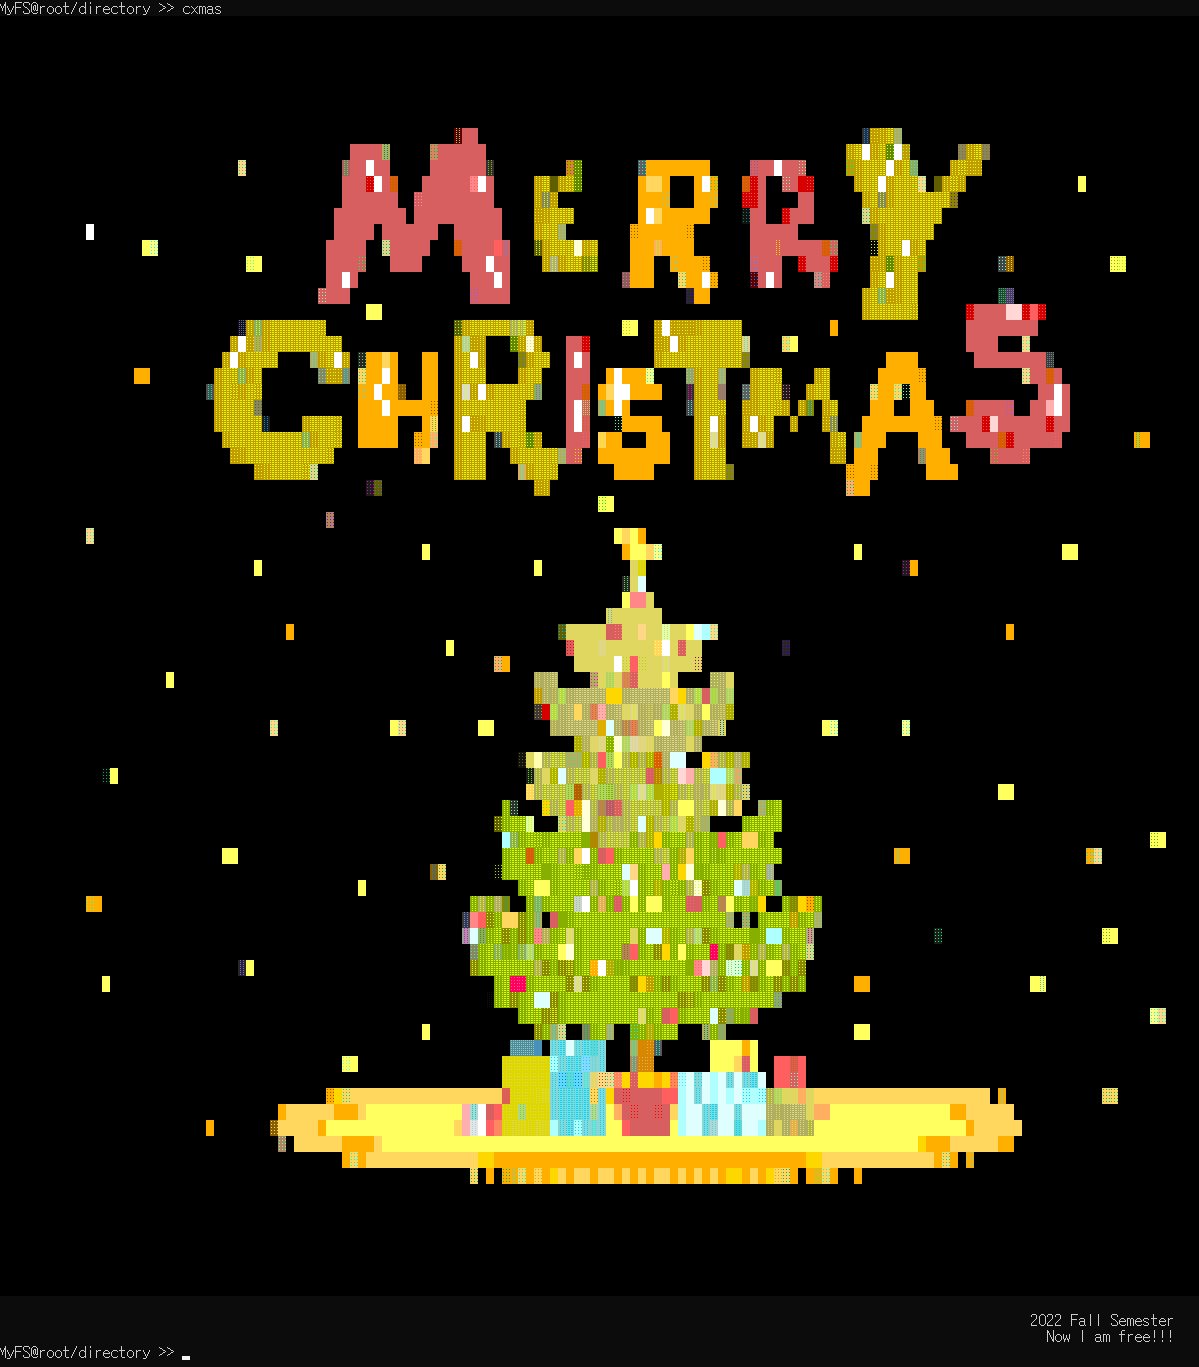
\includegraphics[scale=0.36]{cxmas.png}    
\caption{Colored Christmas Tree}
\end{center}
\end{figure}
\pagebreak

\section{Future Idea \& Conclusion}
\begin{chapquote}{}
          {Richard Feynman}
          ,,What I cannot create, I do not understand.''
\end{chapquote}
We learned file system in the class. In the class time, the concept such as \textit{FAT} seemed to be quite straight forward. Therefore, we thought that project 3 would have been a quite simple implementation. However, that turned out to be completely wrong. This was the longest code throughout the whole semester. As Richard Feynman said, if we could not implement a simple file system, we do not understand the concept completely. Therefore we tried hard to implement the code. To close this report, those are the conclusions and future plans for further topics.
\subsection{Conclusion}
Implementing \texttt{MyFS} was a lot of fun. Since we actually managed to build a simple file system that supports some basic commands, it was satisfying to see them working properly as they should. There were some difficulties with implementations. The following list are the things which we had the most challenges but with the most fun in it.
\subsubsection{Directory Tree}
Since we decided to use "Left Child Right Sibling" tree in order to store the directory structure and for caching the structure, implementing the tree was one of a big huddle. The concept of the tree was quite straight forward. However, with implementing create, delete and moving files, making the directory tree track everything was quite challenging. By implementing this tree based directory system, we were able to learn how to use tree data structure properly.

\subsubsection{Writing Disk}
Since this project were to implement a file system that actually works, we needed to store data into the physical file in our PC. In order to make this work, we had to use lots of \texttt{memcpy}, \texttt{memset}, \texttt{strcpy} and \texttt{malloc}. Not to forget the fact that we actually had to kind of  trick \texttt{C} to think \texttt{struct blocks} as an array of \texttt{unsigned char} for offset calculation. Or treat \texttt{unsigned int} as an array of 4 \texttt{unsigned char} to perform \texttt{memcpy}. Yes, this was super fun. One of the most challenging part when calculating the offset was following code:
\\
\begin{center}
\begin{code}
\begin{minted}[frame=single,framesep=10pt]{C}
...
while (offset <= buffer_size) {
    // Seek throughout the directory file and look for the file name
    char file_name[0x10] = {0};
    memcpy(file_name, buffer + offset + 0x10, sizeof(unsigned char) * 0x10);
    if (!strcmp(file_name, target)) { // Meaning that we have found the name.
        found_target = 1;
        memset(buffer + offset, 0, sizeof(unsigned char) * 0x20); 
        memcpy(buffer + offset, buffer + offset + 0x20, 
               (int) (in->size - offset - 0x20) > 0 ? 
               in->size - offset - 0x20 : 0); 
        break;
    }
    offset = offset + 0x20;
}
...
\end{minted}
\end{code}
\end{center}

This is the code used when we had to rearrange directory file's entries when an entry was removed. Let's assume that we had following files:

\begin{figure}[h]
\begin{center}
\begin{minipage}{7cm}
\dirtree{%
.1 /.
.2 foo.
.2 bar.
.2 baz.
.2 qux.
.2 quux.
}
\end{minipage}
\end{center}
\caption{Example rearranging}
\end{figure}
Suppose that we deleted \texttt{bar}. When we delete \texttt{bar}, there will be an \texttt{0x20} sized offset in the directory file. To avoid having those gaps, we had to shift all entries after \texttt{bar}. As you can see, we have bunch of pointer arithmetic operations to calculate offset and bytes size. Therefore, physically writing disks and calculating those offsets were one of the most challenging parts. After finishing the implementation of this file system project, we were able to calculate offsets and perform memory copies far better than we ever could.

\subsection{Future Idea}
There were lots of great ideas within this \texttt{MyFS} project. Some were successfully implemented, meanwhile some could not. These were the things that we could not implement due to constrains:
\begin{itemize}
    \item \textbf{Mount}: We wanted to implement mounting feature. By treating each \texttt{.img} file as a separate disk, we wanted to make the program mount a specific volume into a directory just like Linux.
    \item \textbf{Device Files}: We wanted to implement a simple device files using file system. For example, we wanted to perform some actions like \texttt{write /dev/screen "hello world"} print out \texttt{hello world} into the screen. Or perform give some other device files to interact with.
    \item \textbf{Strict Permissions}: We wanted to make a multi-user environment. Since our file system supports permissions, we wanted to put strict permissions on each files. That is, some user has access to a specific file, when some does not.
    \item \textbf{Real Indirection}: Since the original file system had size limit of 6 disk blocks, we wanted to create an indirection table that can make a single file much bigger.
\end{itemize}
These ideas were the things we tried to implement in \texttt{MyFS} at first, however was not able to. Beside those ideas, there are some other good topics we also wanted to implement. To list a few:
\begin{itemize}
    \item \textbf{RAID}: As we have mentioned before, creating an RAID file system was one of our first goals. As inspired by the mid-term's final question (the 50 points one), we wanted to implement the RAID 0 system and compare the performance between just using one disk. Then make a statistical report on how better it performed. Not only the RAID 0, but also those RAID 3 and 4 that supports parity. Also with RAID 0 and RAID 3 combined for better reliability as well.
    \item \textbf{Disk Generator}: As suggested in the original guide line that professor gave us, we wanted to create a disk generator that generates disk images randomly and correctly. Not only we wanted the disk images, we also wanted to implement some bigger file system generator. Since our file system has limitations of 4 megabytes, we wanted to make a program that actually writes bigger disk images and works across the bigger disk.
\end{itemize}
Those future ideas are still in our mind and would like to implement more features in the future when we have spare time.

\subsection{Final Conclusion}
Throughout this semester, we had learned following things:
\begin{itemize}
    \item \textbf{Introduction to OS}: About threads, concurrency, multi-processes.
    \item \textbf{Scheduling}: About scheduling techniques and its metrics, such as round robin, CFS, and etc.
    \item \textbf{Virtual Memory}: About virtual addresses and its usages, such as shared memory, page table, swapping and etc.
    \item \textbf{File System}: About storing files and its applications.
\end{itemize}
We learned a lot. Throughout this semester, as we have implemented various projects and assignments, we learned following things:

\begin{itemize}
    \item \textbf{Trade-off}: In operating systems, there is no such thing like "answers". For example, if foo is better than bar in terms of a, in the most cases bar is better than foo in terms of b. Round robin gives us fast response time compared to FIFO. However, FIFO gives us faster turnaround time than round robin. We learned that OS is balancing in the middle and selecting reasonable trade-offs that will work the best. Since there was no such thing like "answers", OS was an interesting subject to study.
    \item \textbf{Insight}: Before learning operating systems, we were very short sighted and saw a single tree, not the forest. After learning operating systems, we kind of got knowledge about how things work in a overall system. For example, multi-threading is good. Before getting insights about operating systems, we all thought making a multi-threaded program will always perform better. However, after the class, instead of blindly saying that something is better than something, we started to question ourselves on "is this really better?". For example, with poorly designed multi-threaded program, it will perform worse than single threaded.
\end{itemize}
It was a great joy of implementing almost everything that we had learned throughout the class. By projects, we were able to understand topics clearer. This was a great class. We will be closing our report here.
\end{document}
